\documentclass{article}
\usepackage{amsmath}
\usepackage{graphicx}
\usepackage{listings}
\newcommand{\includecode}[2][c]{\lstinputlisting[caption=#2, escapechar=, language=#1]{#2}}

\begin{document}
\lstset{language=C} 
\title{Introducing periodic boundary conditions in a Molecular Dynamics simulation}
\author{Alexander Wagner}
\maketitle
\begin{abstract}
 We show how in a molecular simulation particles can be contained in a bulk-like environment by using periodic boundary conditions. In this report we focus on how such boundary conditions are implemented in detail in a Molecular Dynamics code.
\end{abstract}

\section{Introduction}
In this report we are focusing on simulations of molecular systems. The particles move under classical Newtonian dynamics and are represented as coordinates and velocities. Typically only a small part of such a system can be represented in a simulation. To simulate such a bulk system, it is important that particles in a simulation are contained. The most obvious solution would be to define a container that keeps the particles in place. However, doing so would introduce special boundary effects, that can differ substantially from bulk behavior. Periodic boundary conditions are an effective way of containing the particles without introducing boundary effects. The rest of the report is structured as follows: first we introduce the theory behind periodic boundary conditions, then we explain how this can be implemented in a code. We then demonstrate that the code manages to contain the particles. We also comment on situations in which this code can fail. We conclude that, as long as sensible parameters are chosen that will prevent very large jumps of particles, our code performs well. The full code is presented in an appendix.

\begin{figure}
  \begin{center}
    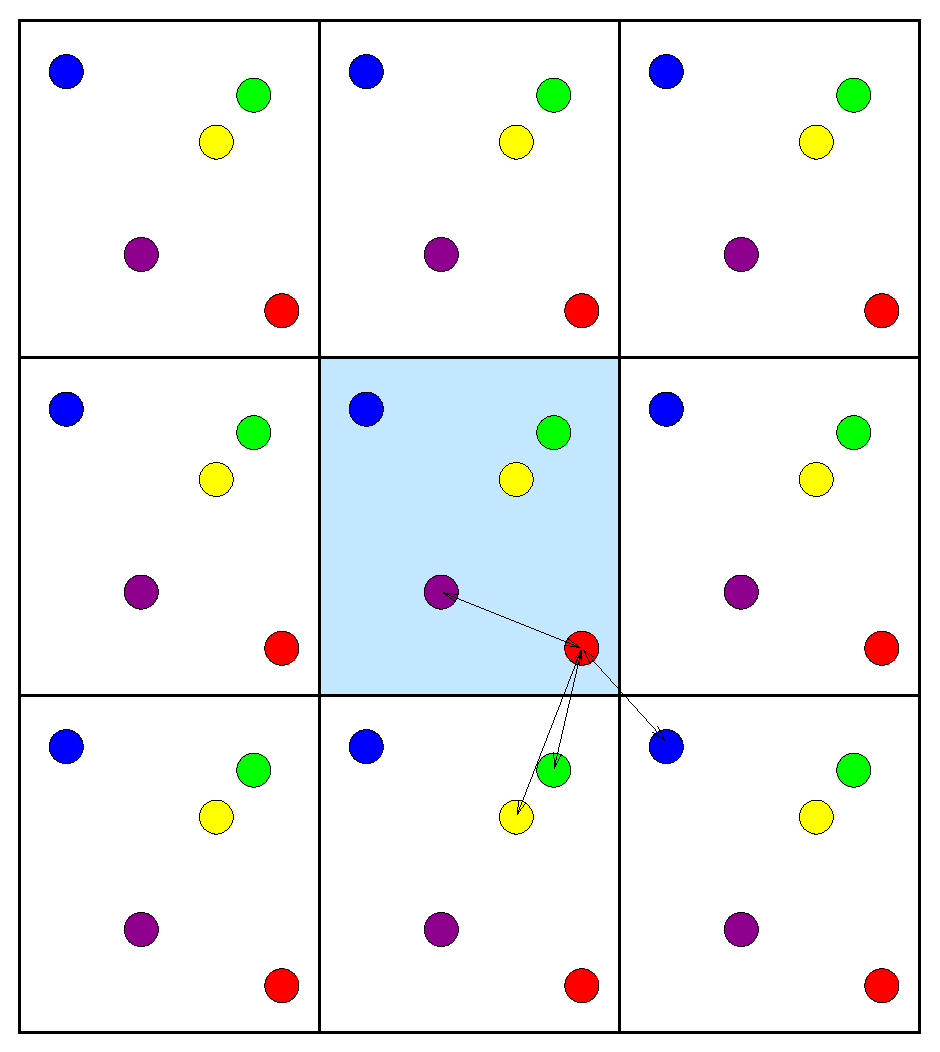
\includegraphics[width=0.5\textwidth]{Periodic.eps}
  \end{center}
  \caption{\label{fig1}A sketch of the idea behind periodic boundary conditions. The modeled system consists only of the slightly darker middle square. However, particles will interact with the closest periodic image, in stead of the actual particle if those are closer.}
\end{figure}

\section{Periodic boundary conditions}
The idea behind the periodic boundary conditions are shown in Figure \ref{fig1}. The system is seen as extending to infinity, but in an entirely periodic manner. Particles interact not only within the simulation cell, but also with all periodic images of these particles. For this to be practical it is usually assumed that the interactions fall of quickly with distance, so that only one interaction with the closes image has to be taking into account. This also means that only one shell of periodic images around the original system has to be taken into account.

Our molecular dynamics code implements Newton's equations
\begin{align}
  \dot{\mathbf{x}}_i = \mathbf{v}_i\\
  \dot{\mathbf{v}}_i = \frac{\mathbf{F}_i}{m}
\end{align}
where $\mathbf{x}_i$ is the position vector of the $i$th particle, and $\mathbf{v}_i$ is its velocity. The dot indicates a time derivative, as usual. We discretized this using the Verlet algorithm as
\begin{align}
  \mathbf{v}(t+\Delta t/2)&=\mathbf{v}(t-\Delta t/2) +\frac{\mathbf{F}(t)}{m}\Delta t\\
  \mathbf{x}(t+\Delta t) &= \mathbf{x}(t)+ \mathbf{v}(t+\Delta t/2)
\end{align}
The force is given as a sum of pair forces as
\begin{equation}
  \mathbf{F}_i = \frac{\partial V(\{\mathbf{x}_n\})}{\partial \mathbf{x}_i}
\end{equation}
where the partial derivative here is the same as the nabla operator for the coordinates of the $i$th particle. $V$ is the potential energy of the system, that depends on the coordinates of all the particles. An explicit implementation of this algorithm is given in the appendix. 

Explicitly the function $F$ in the code in the appendix calculates the distances in each dimension, and only retains information about the shortest distance:

\begin{lstlisting}[frame=single]
  double dr[D],dR=0;
  for (int d=0; d<D; d++){
    dr[d]=x[m][d]-(x[n][d]-L);
    double ddr;
    ddr=x[m][d]-(x[n][d]);
    if (fabs(ddr)<fabs(dr[d])) dr[d]=ddr;
    ddr=x[m][d]-(x[n][d]+L);
    if (fabs(ddr)<fabs(dr[d])) dr[d]=ddr;
    dR+=dr[d]*dr[d];
  }
\end{lstlisting}
where $dr[d]$ encodes the $d$th component of the displacement vector between the $n$th and the $m$th particle and $dR$ is the absolute squared of the $\mathbf{dr}$ vector. 

This code fragment shows how we determine the shortest distance between the $n$th and the $m$th particle and their periodic images in $D$ dimensions. This shortest distance is then used in the usual force routine.

The second part of the code that needs to consider periodic boundary conditions is the part where the particle positions are updated. Since we now insist that the particles are contained in a domain from $x_{i\alpha}\in[0,L]$, where $\alpha$ refers to any of the dimensions considered in the code. When a particle leaves this domain one of its periodic images will enter the simulation domain at the same time. The position coordinates are now replaced with the coordinates of the periodic image that happens to reside inside the computational domain. In code, this is accomplished by

\begin{lstlisting}[frame=single]
  x[n][d]+=v[n][d]*dt;
  if (x[n][d]<0) x[n][d]+=L;
  else if (x[n][d]>=L) x[n][d]-=L;
\end{lstlisting}

This completes the implementation of periodic boundary conditions in our Molecular Dynamics code. 

\section{Results}
We tested the algorithm by setting up particles in a regular two-dimensional lattice and giving the particles on the left side an upward velocity of 1 and the right side a downward velocity of -1. The results are shown in Fig. \ref{fig2}.

\begin{figure}
  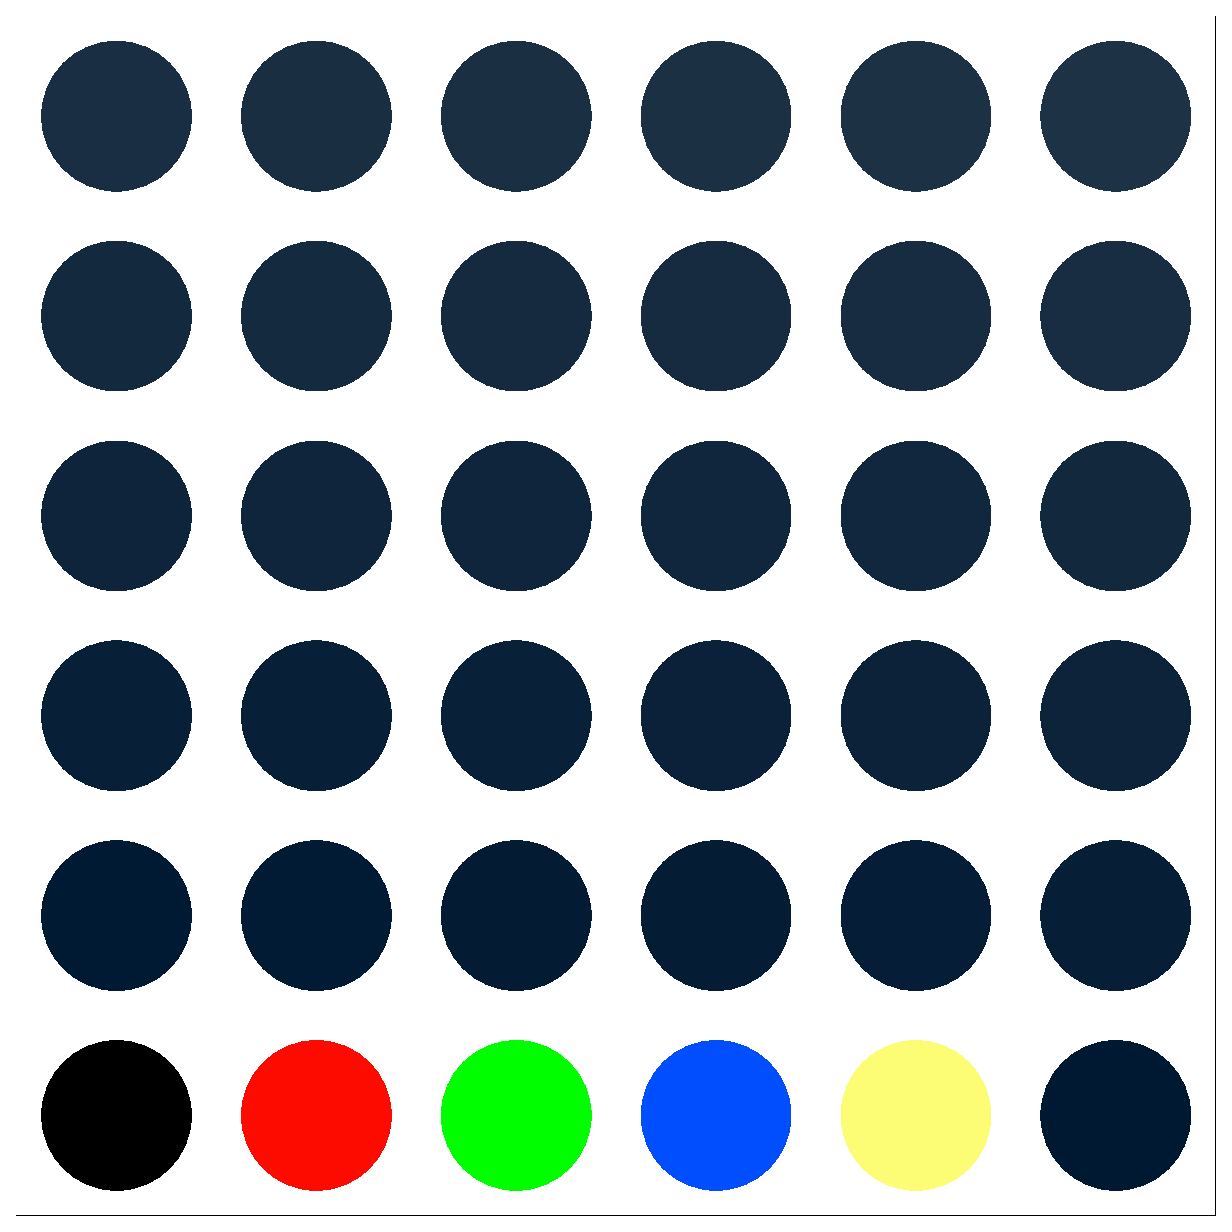
\includegraphics[width=0.19\textwidth]{graph3d_002.eps}
  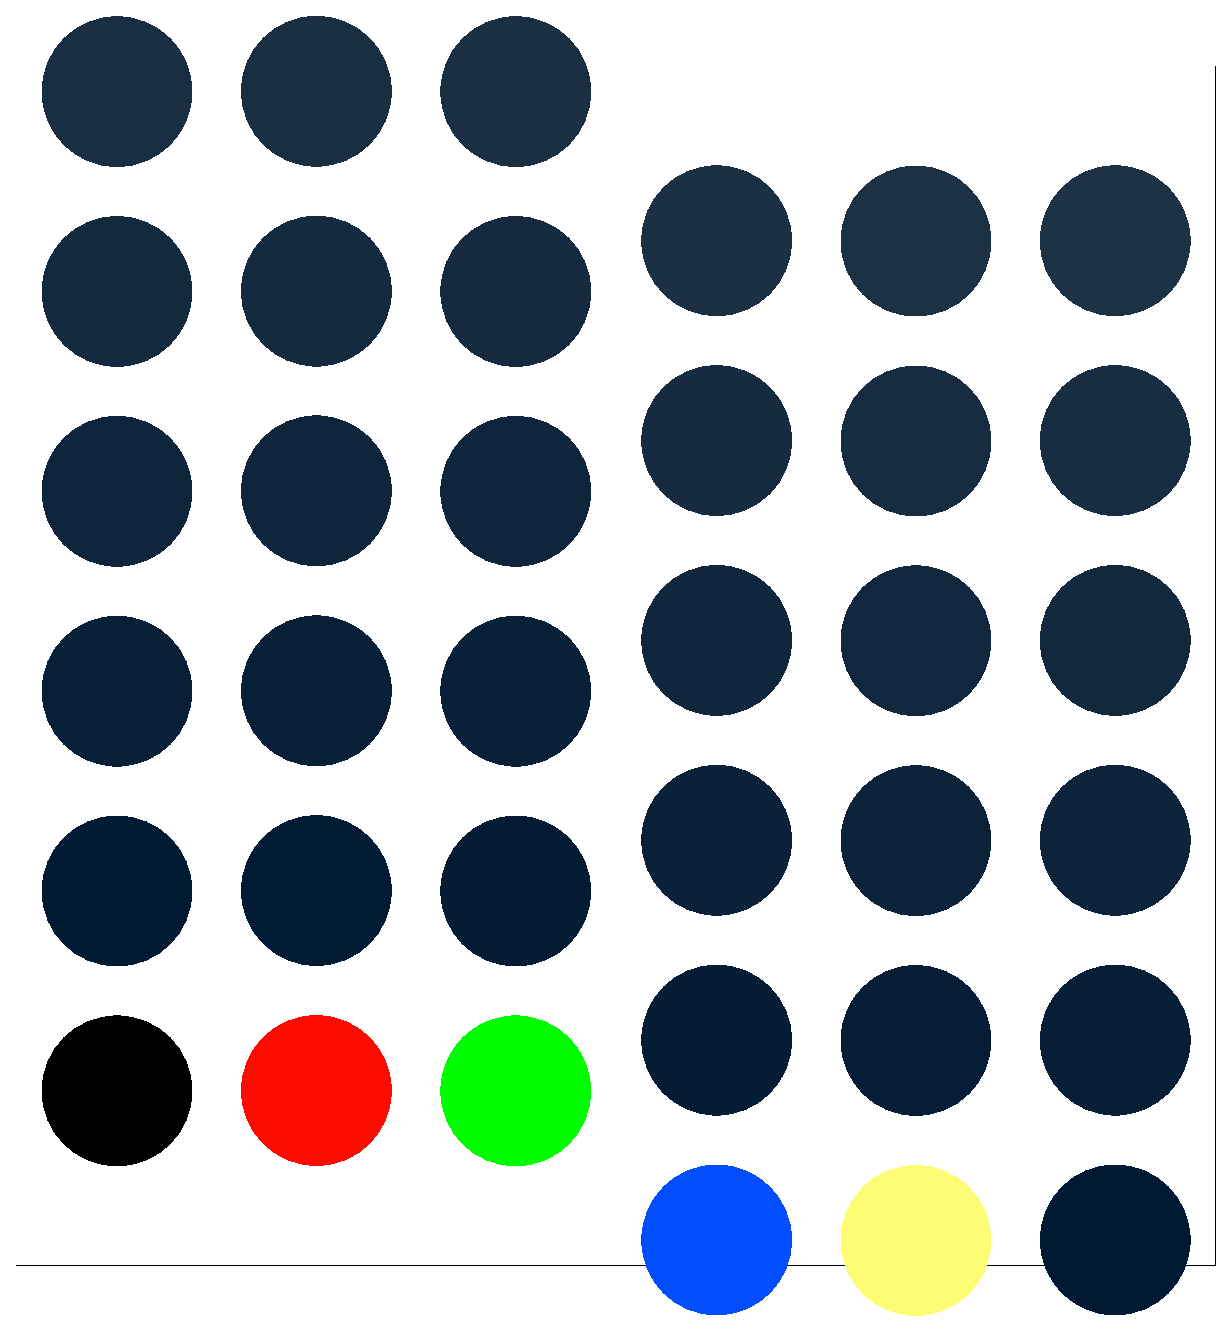
\includegraphics[width=0.19\textwidth]{graph3d_003.eps}
  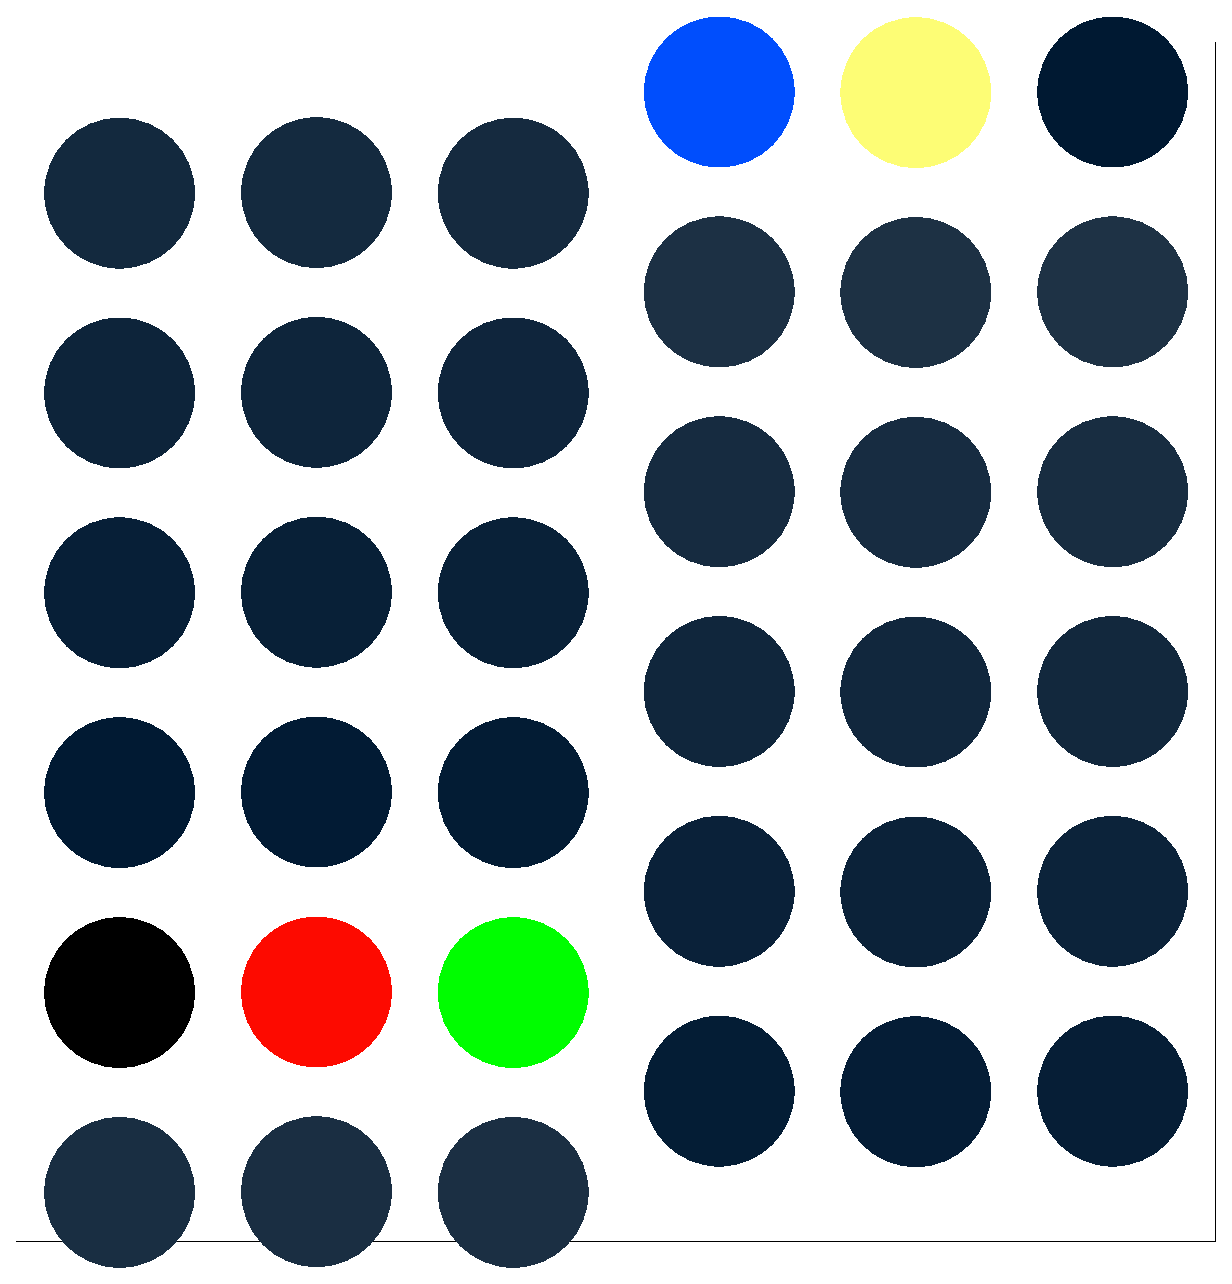
\includegraphics[width=0.19\textwidth]{graph3d_004.eps}
  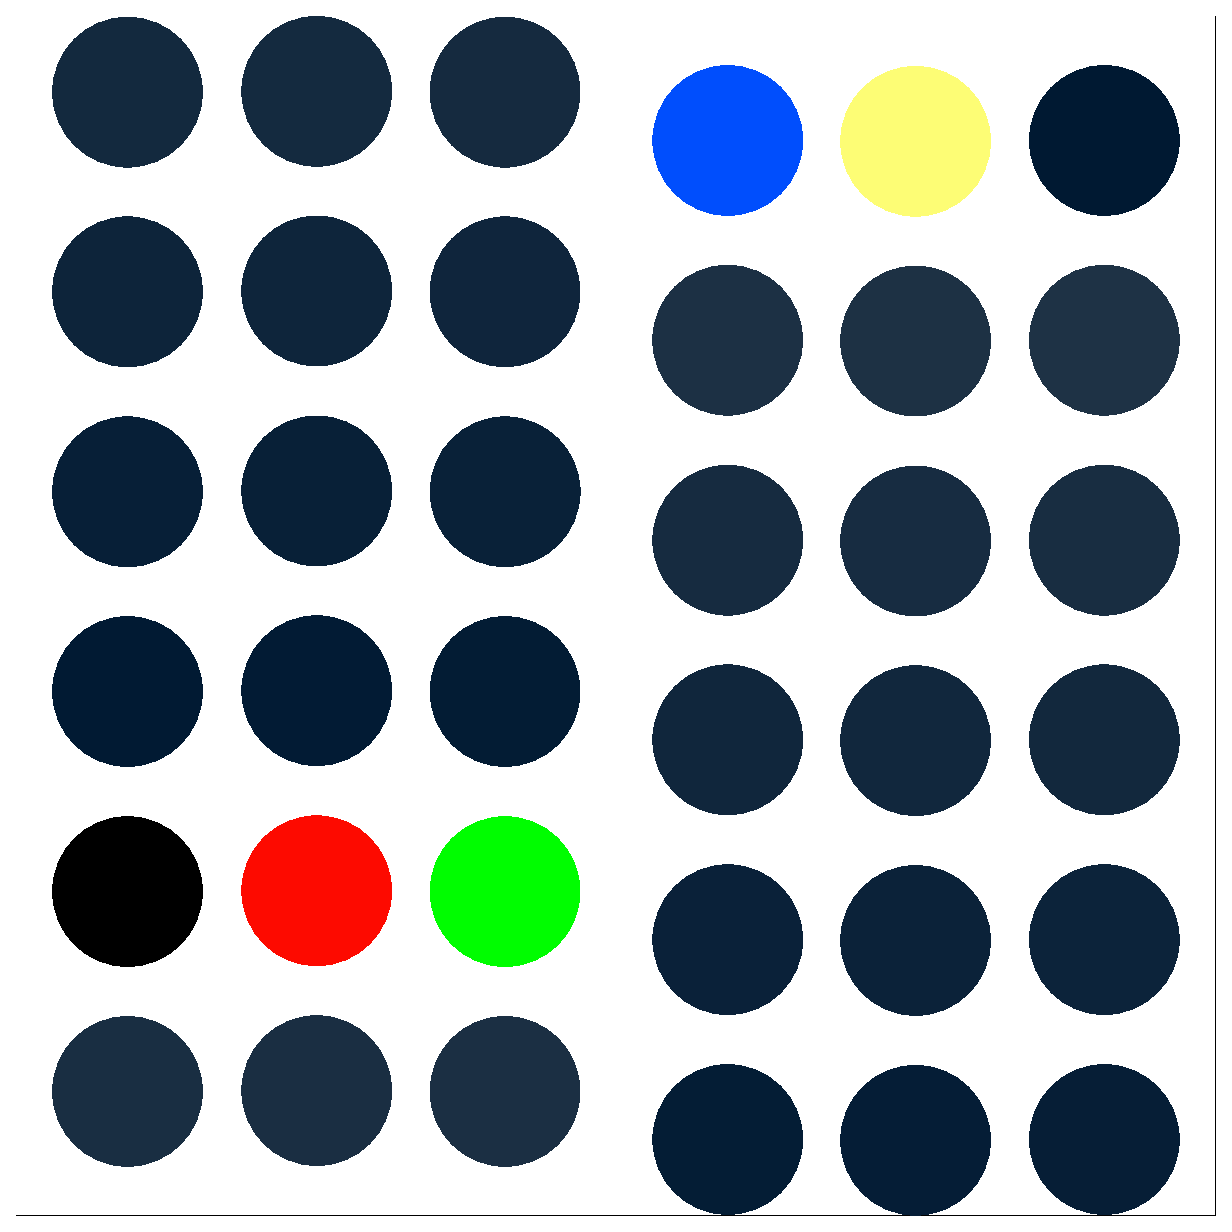
\includegraphics[width=0.19\textwidth]{graph3d_005.eps}
  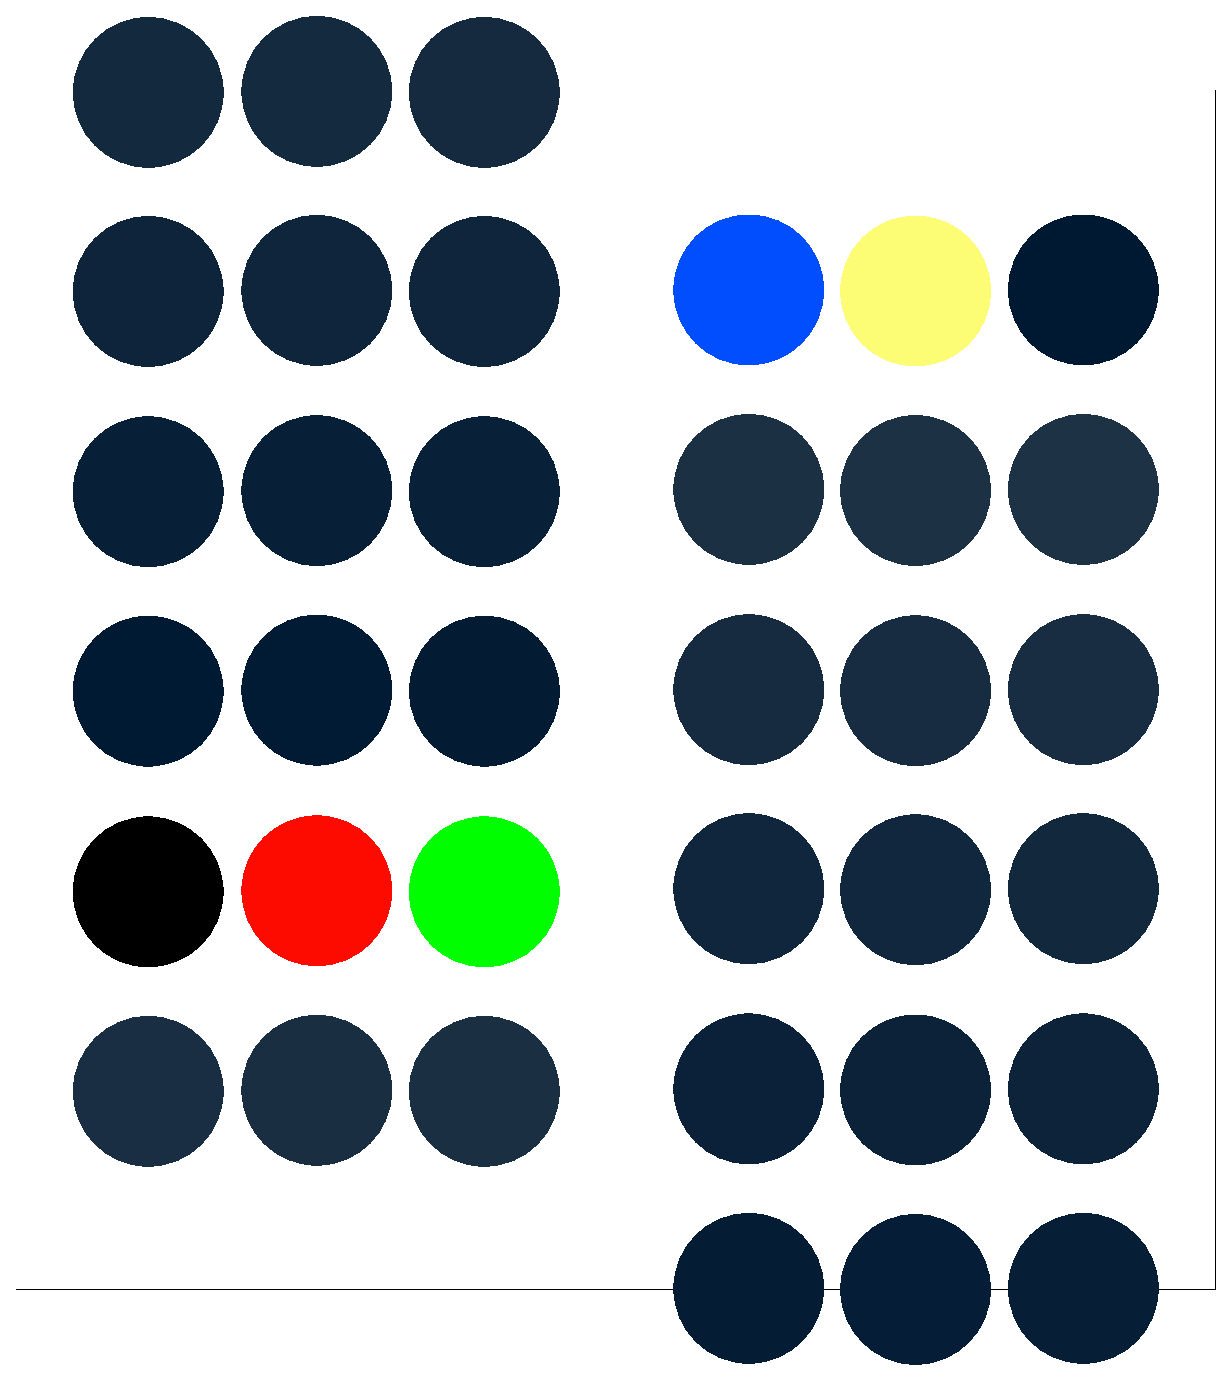
\includegraphics[width=0.19\textwidth]{graph3d_006.eps}
  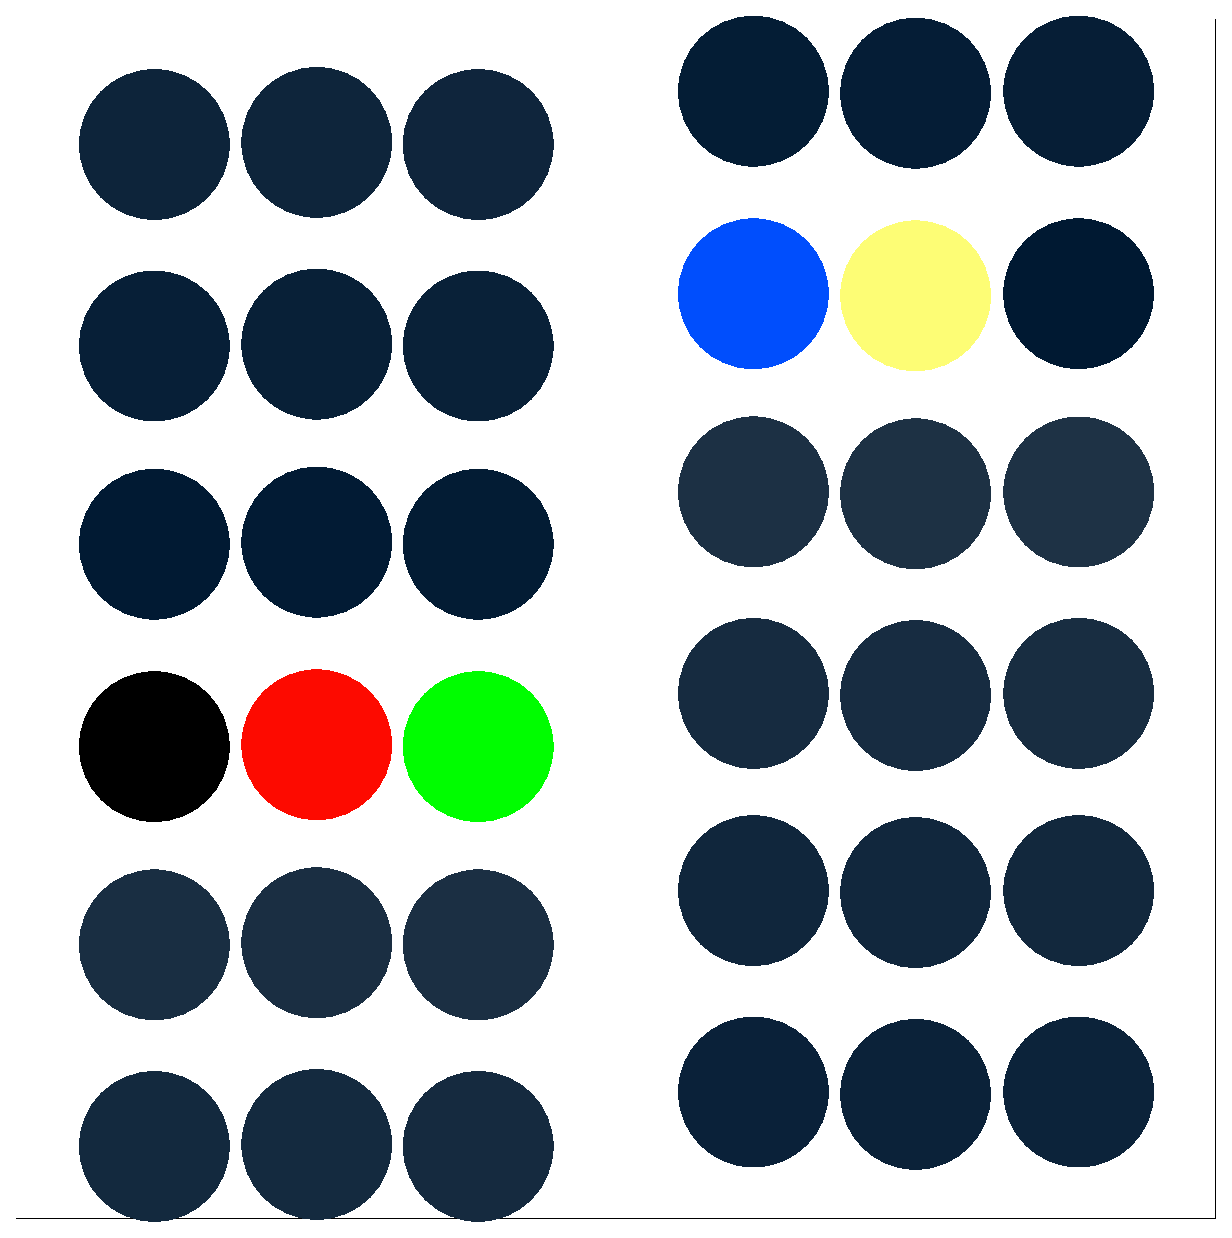
\includegraphics[width=0.19\textwidth]{graph3d_007.eps}
  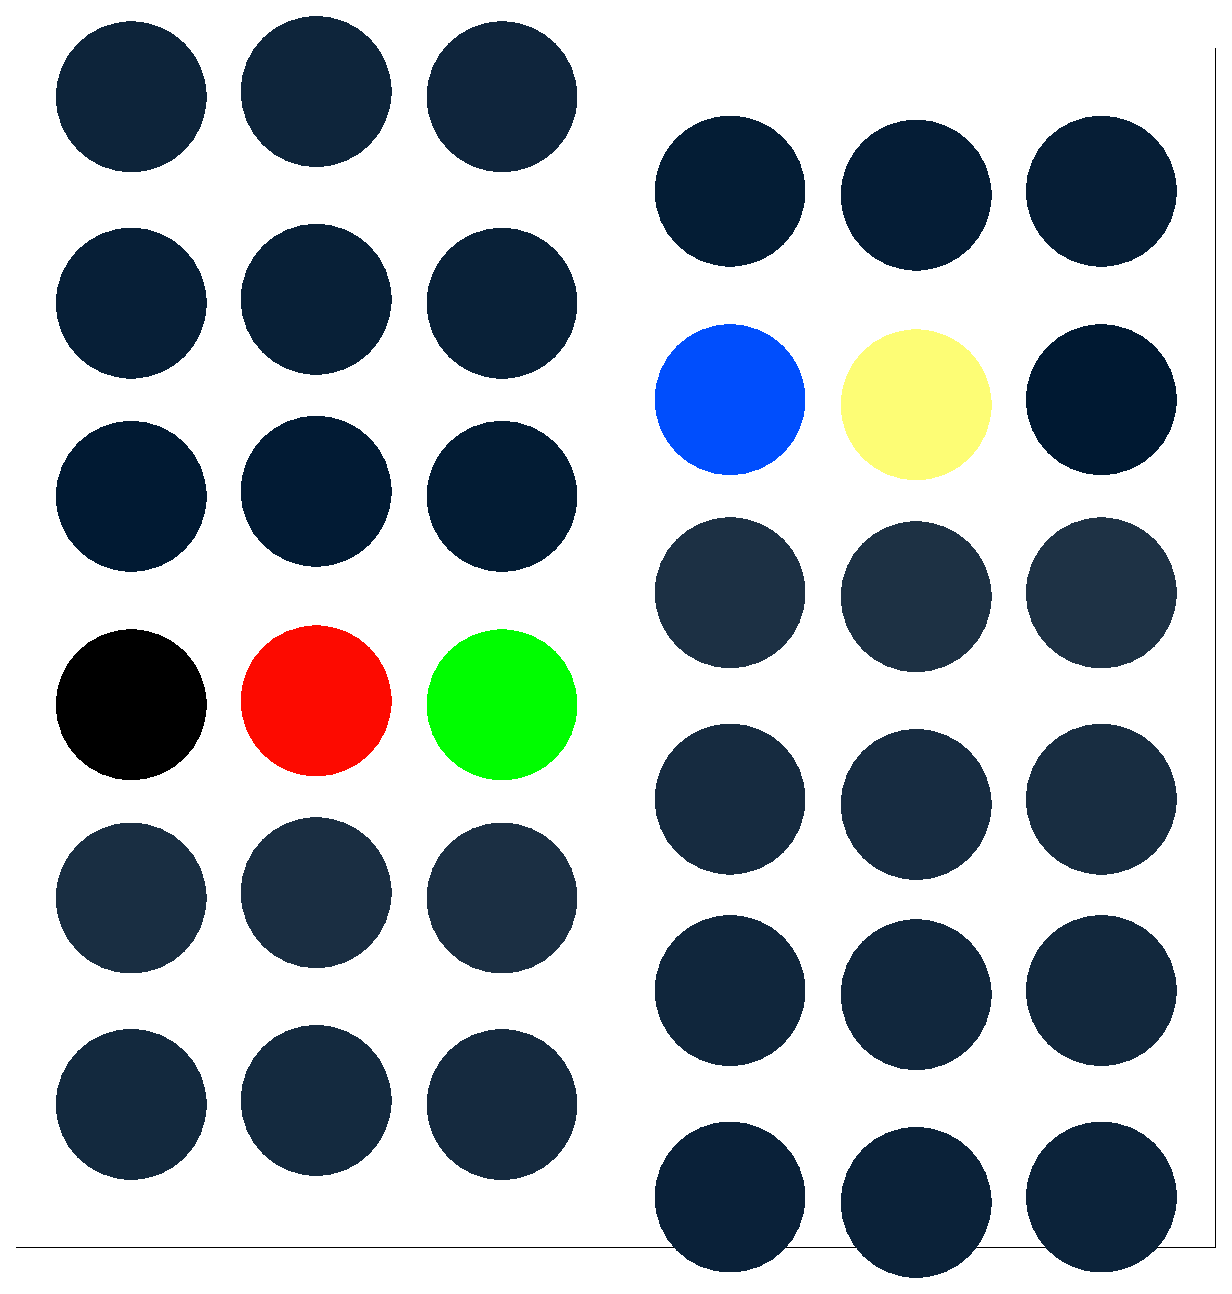
\includegraphics[width=0.19\textwidth]{graph3d_008.eps}
  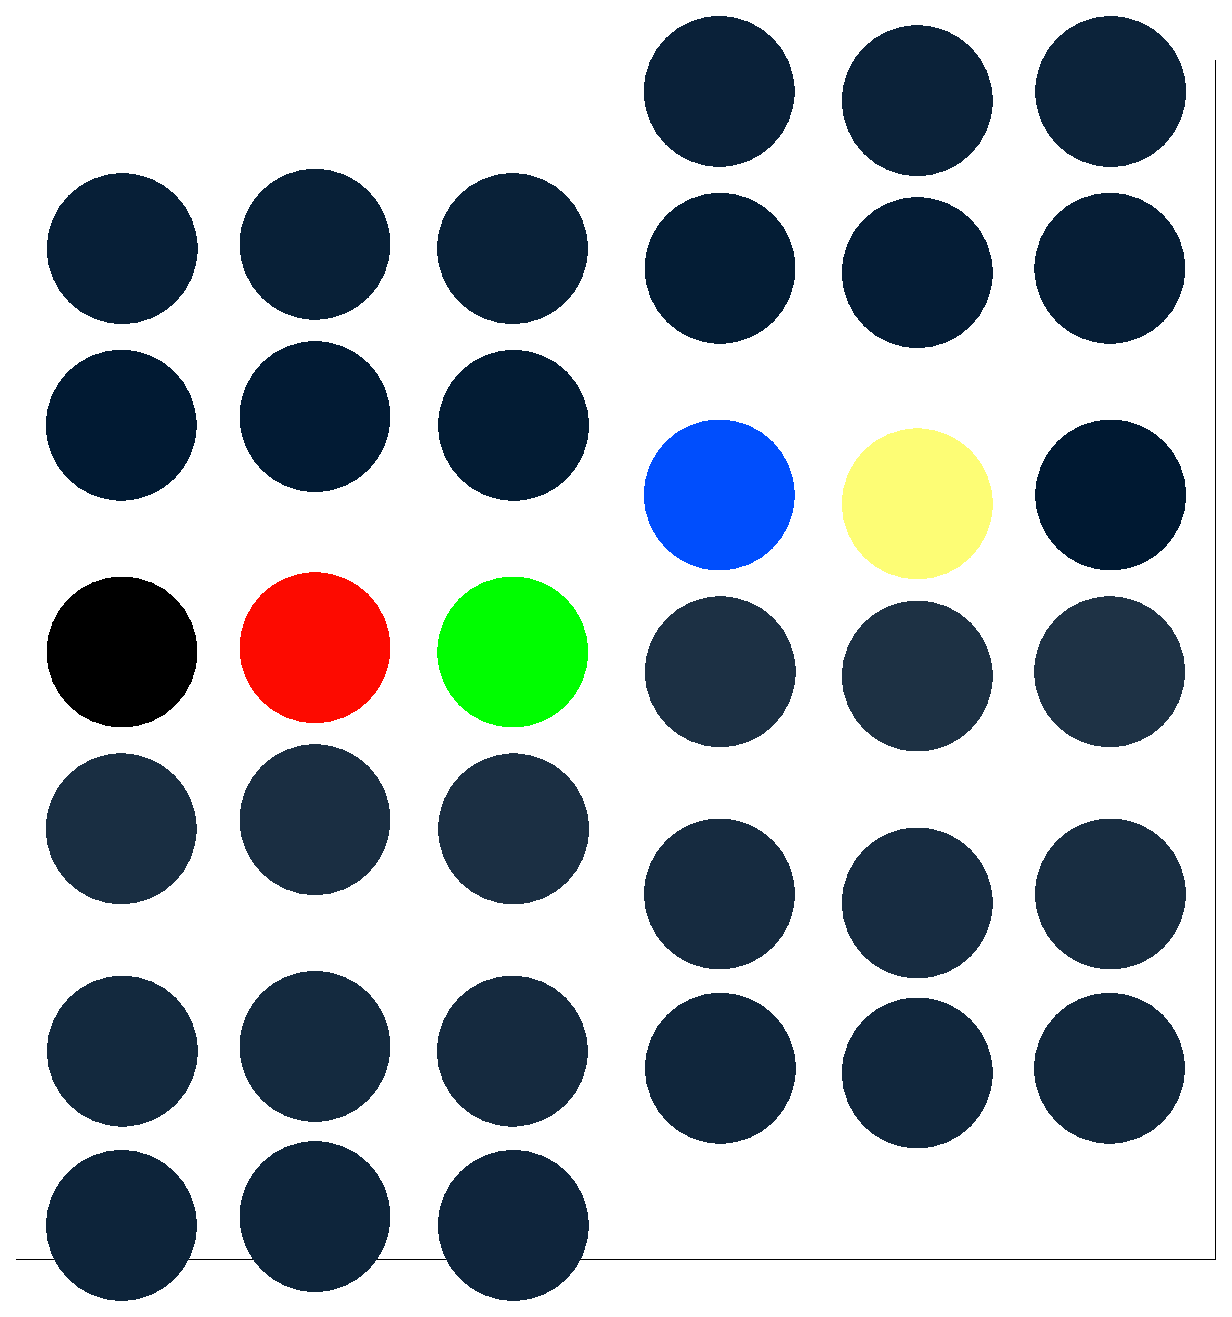
\includegraphics[width=0.19\textwidth]{graph3d_009.eps}
%  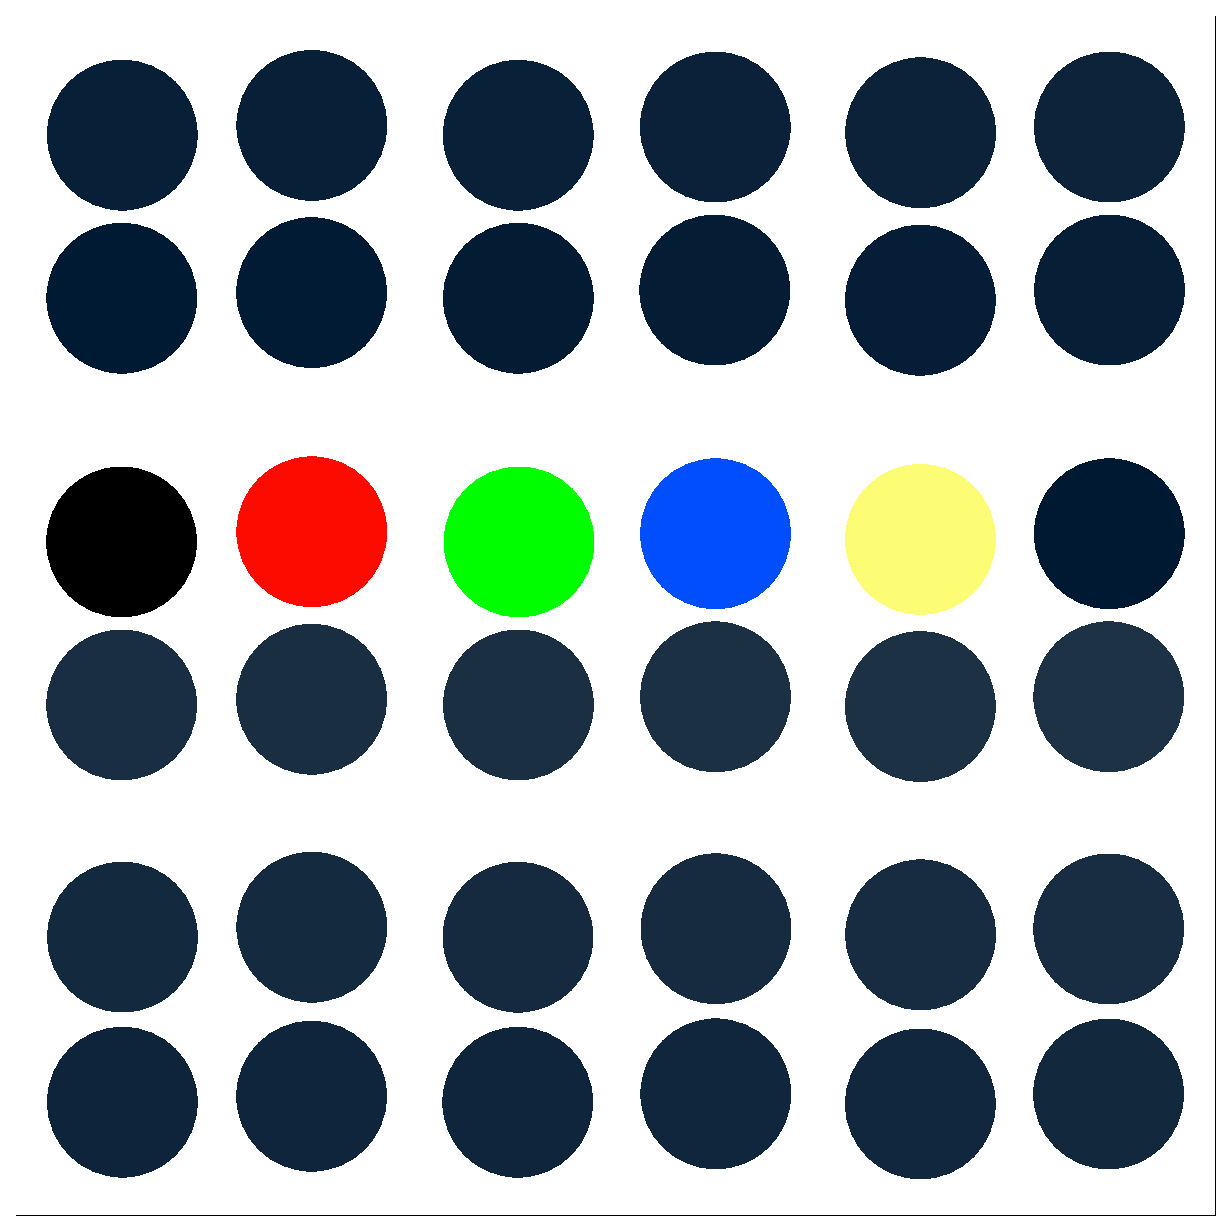
\includegraphics[width=0.19\textwidth]{graph3d_010.eps}
  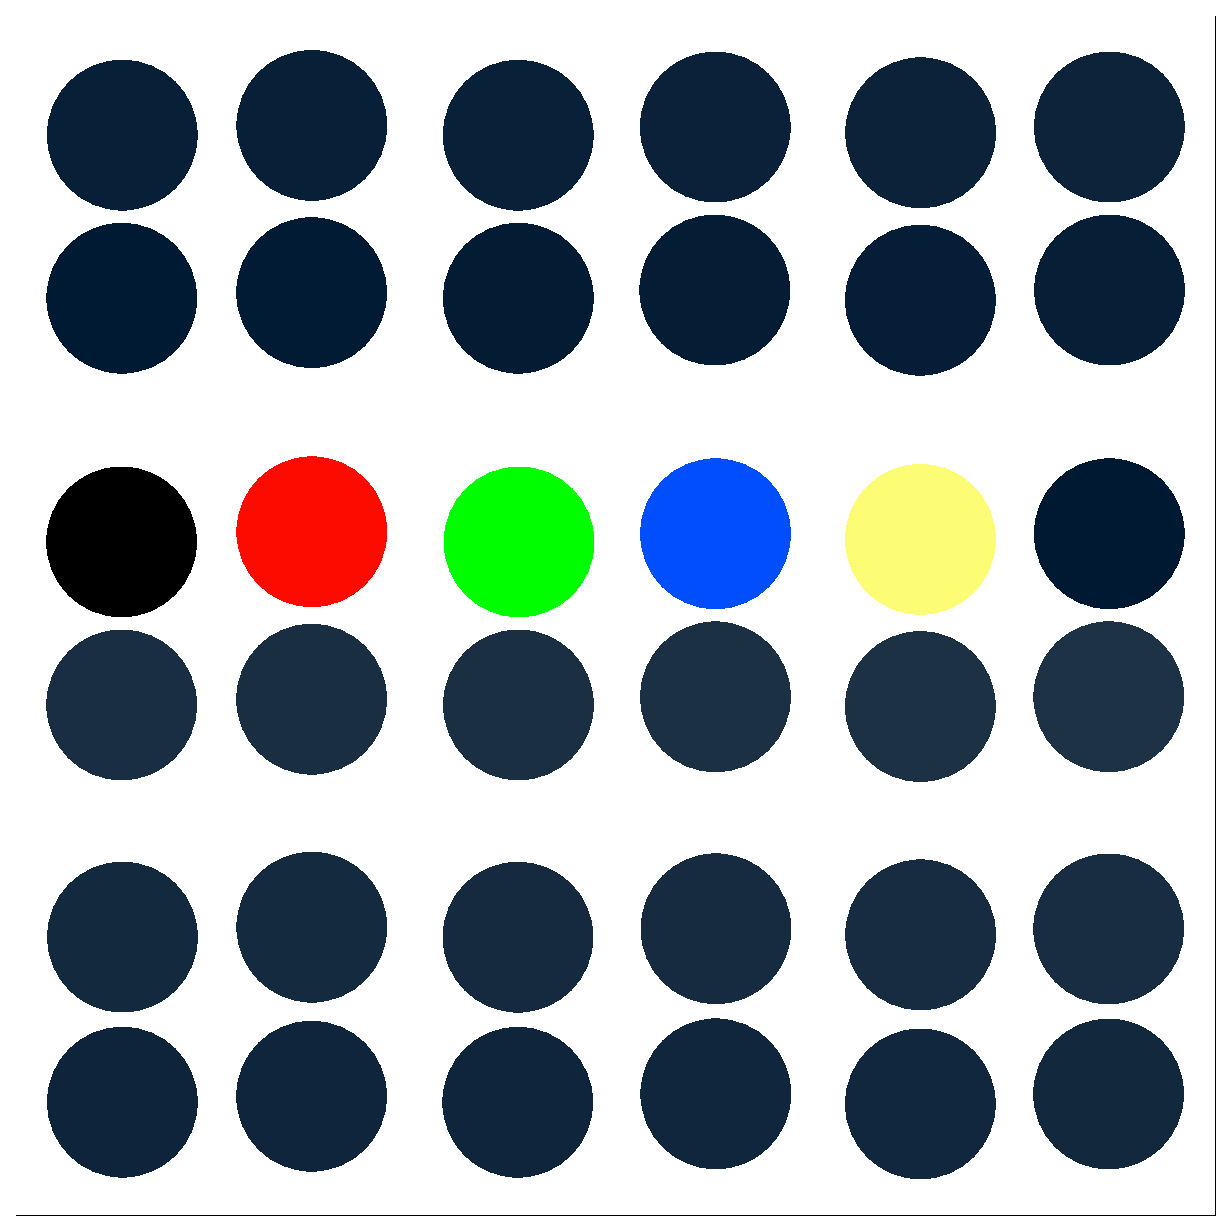
\includegraphics[width=0.19\textwidth]{graph3d_011.eps}
  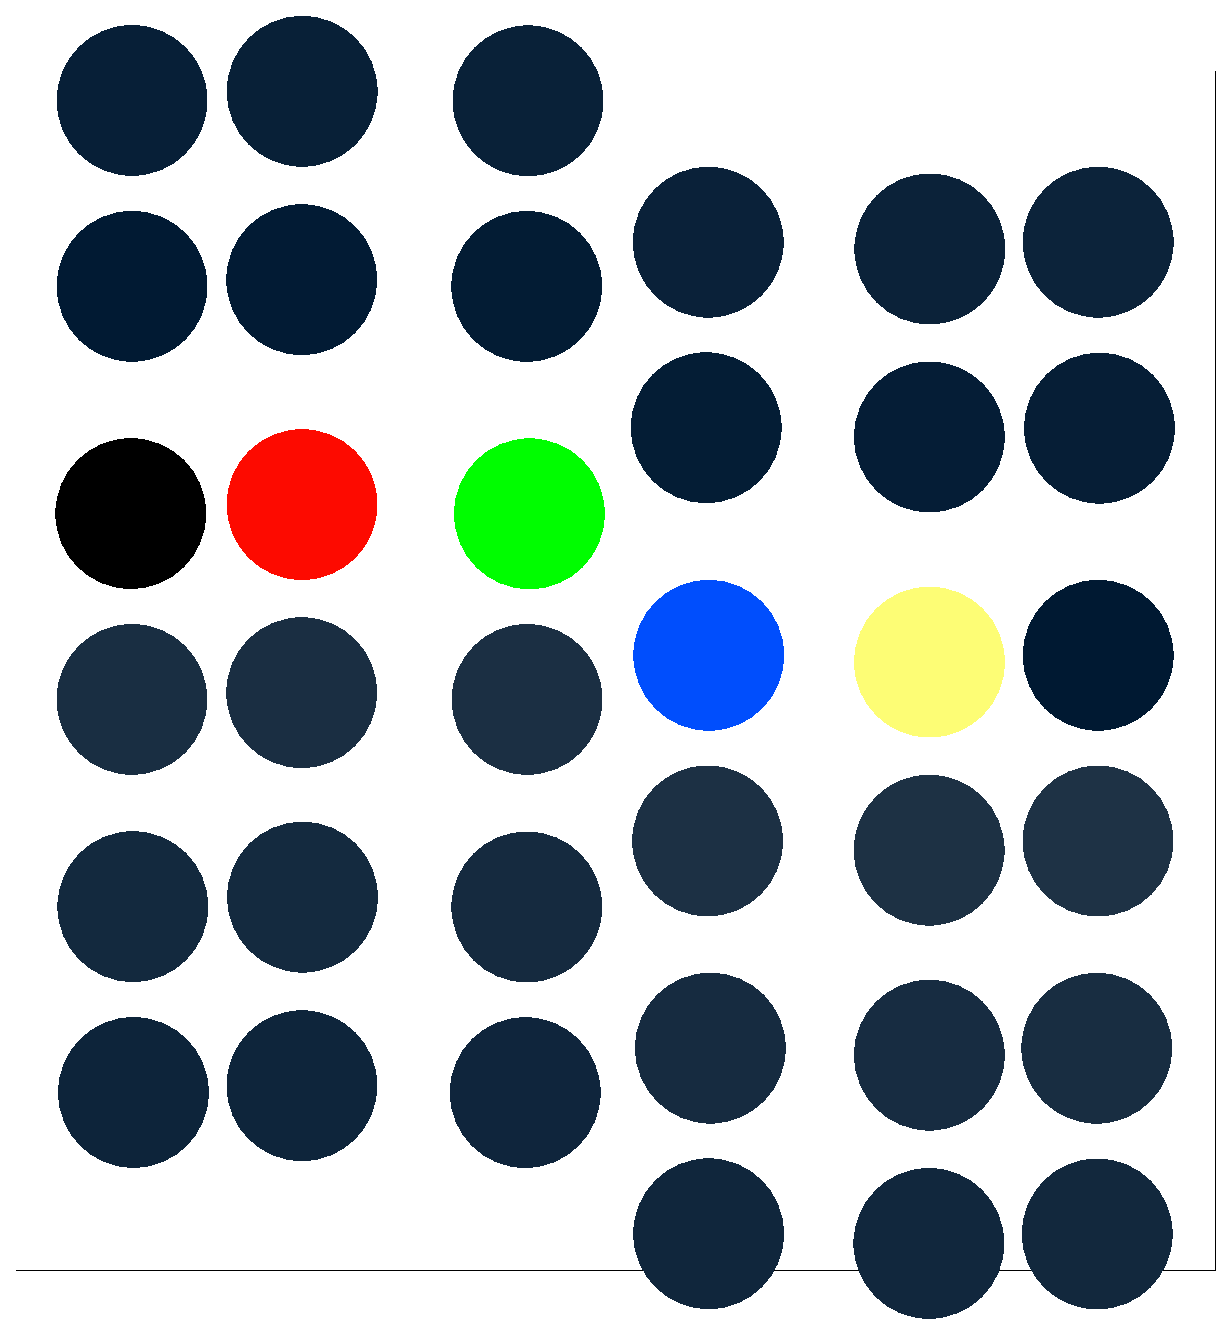
\includegraphics[width=0.19\textwidth]{graph3d_012.eps}
  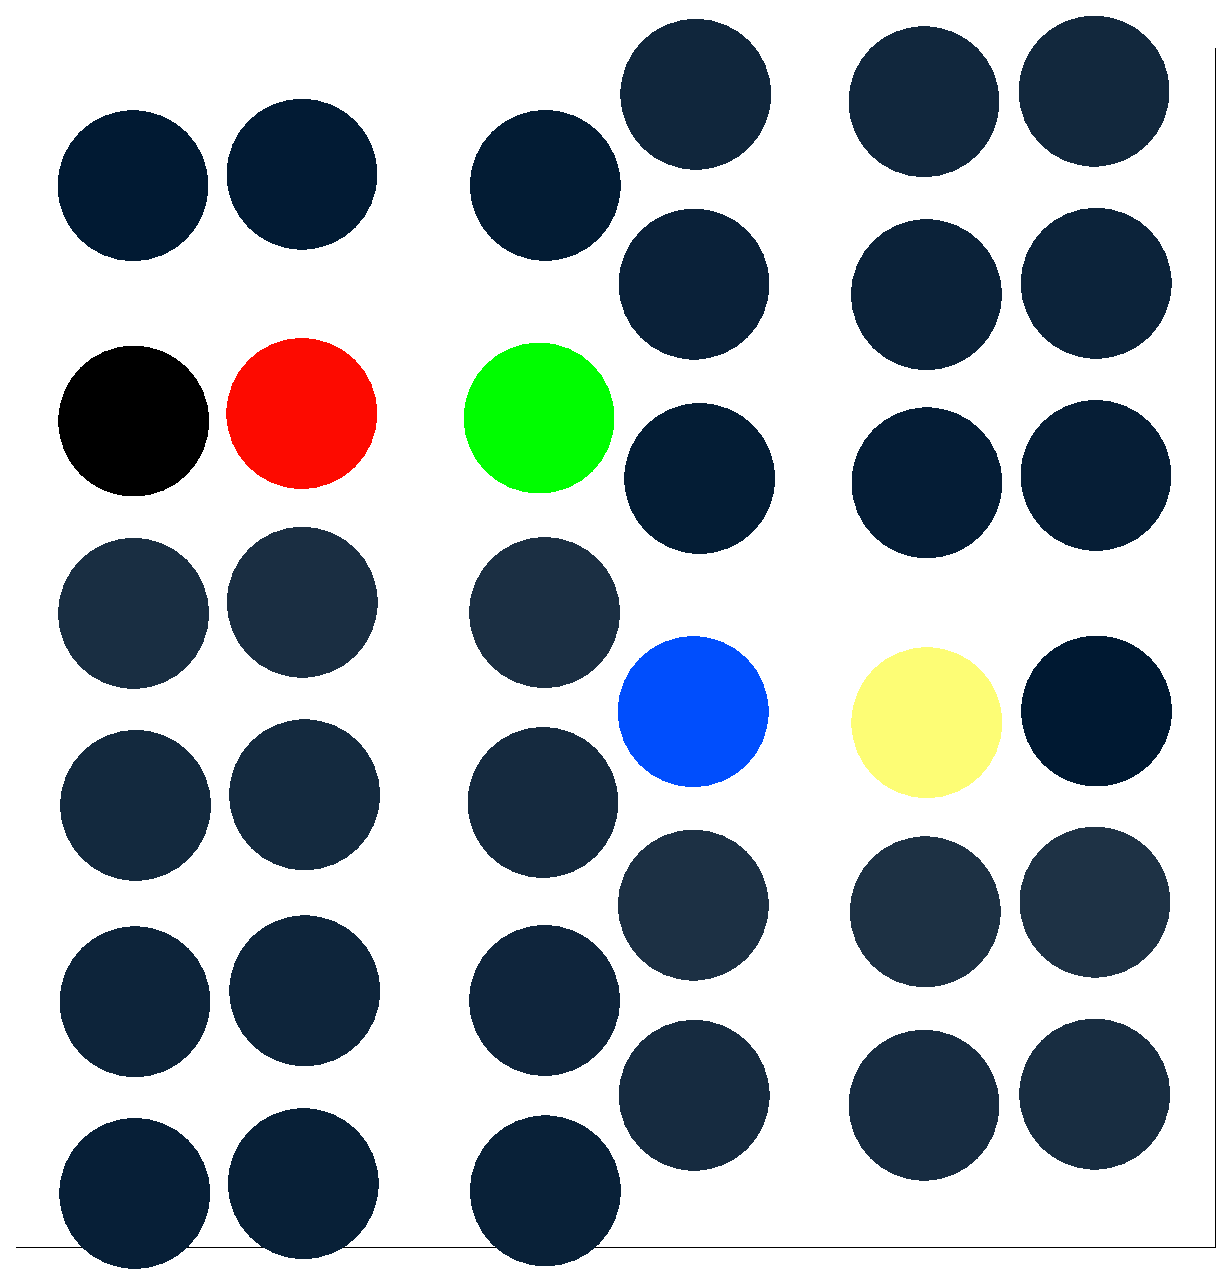
\includegraphics[width=0.19\textwidth]{graph3d_013.eps}
  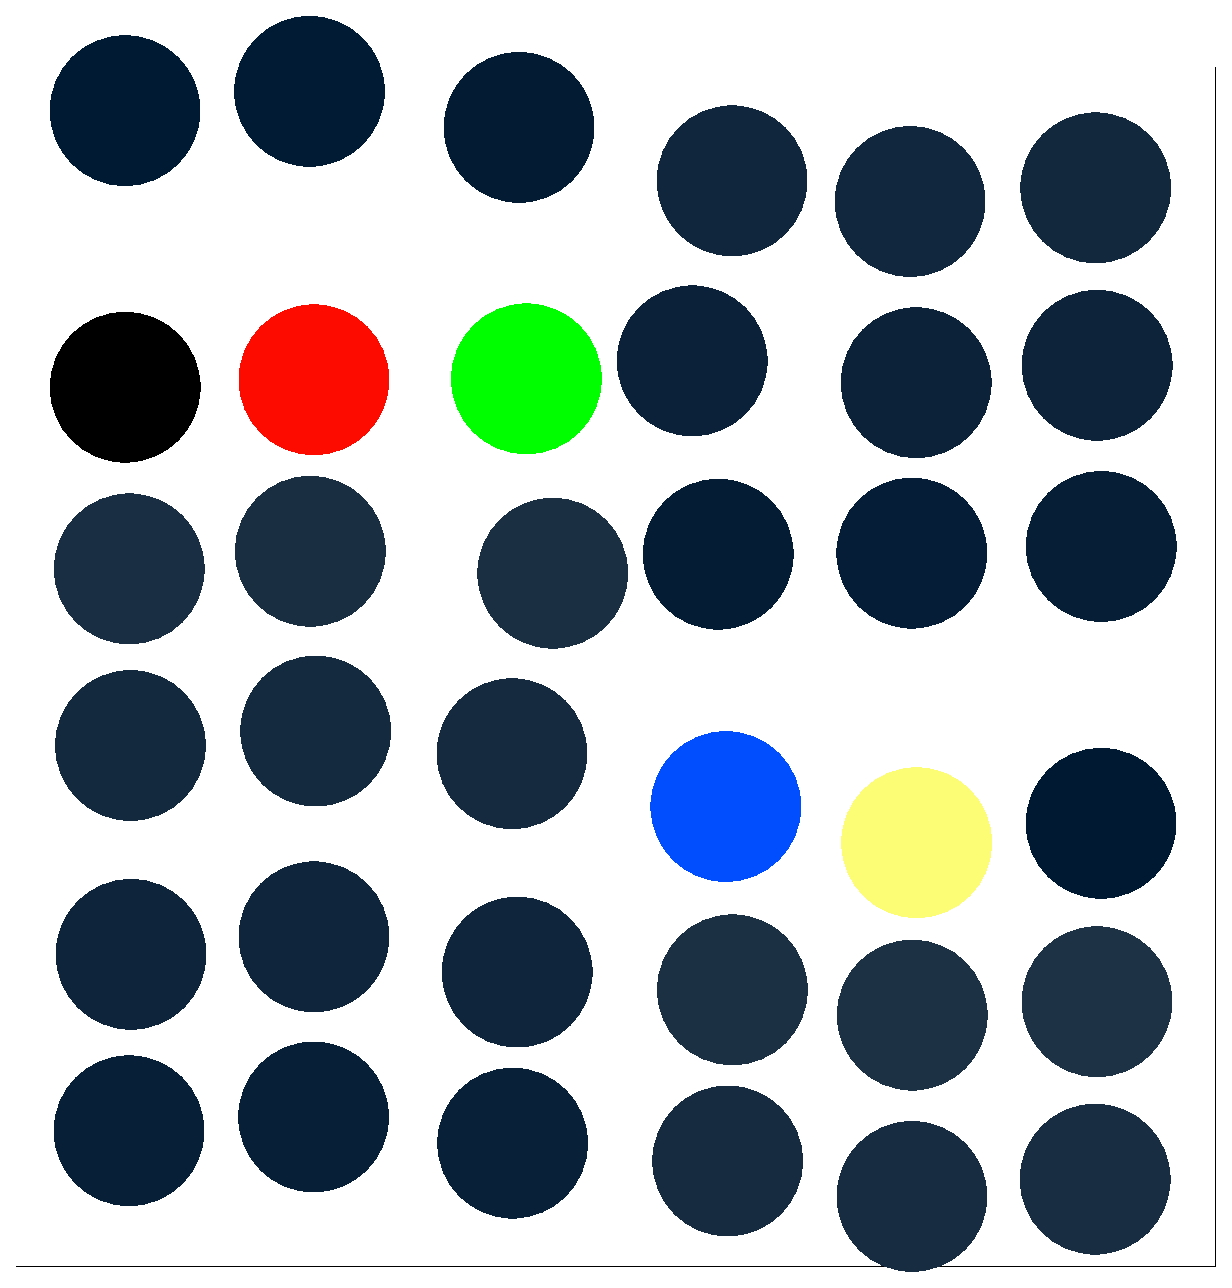
\includegraphics[width=0.19\textwidth]{graph3d_014.eps}
  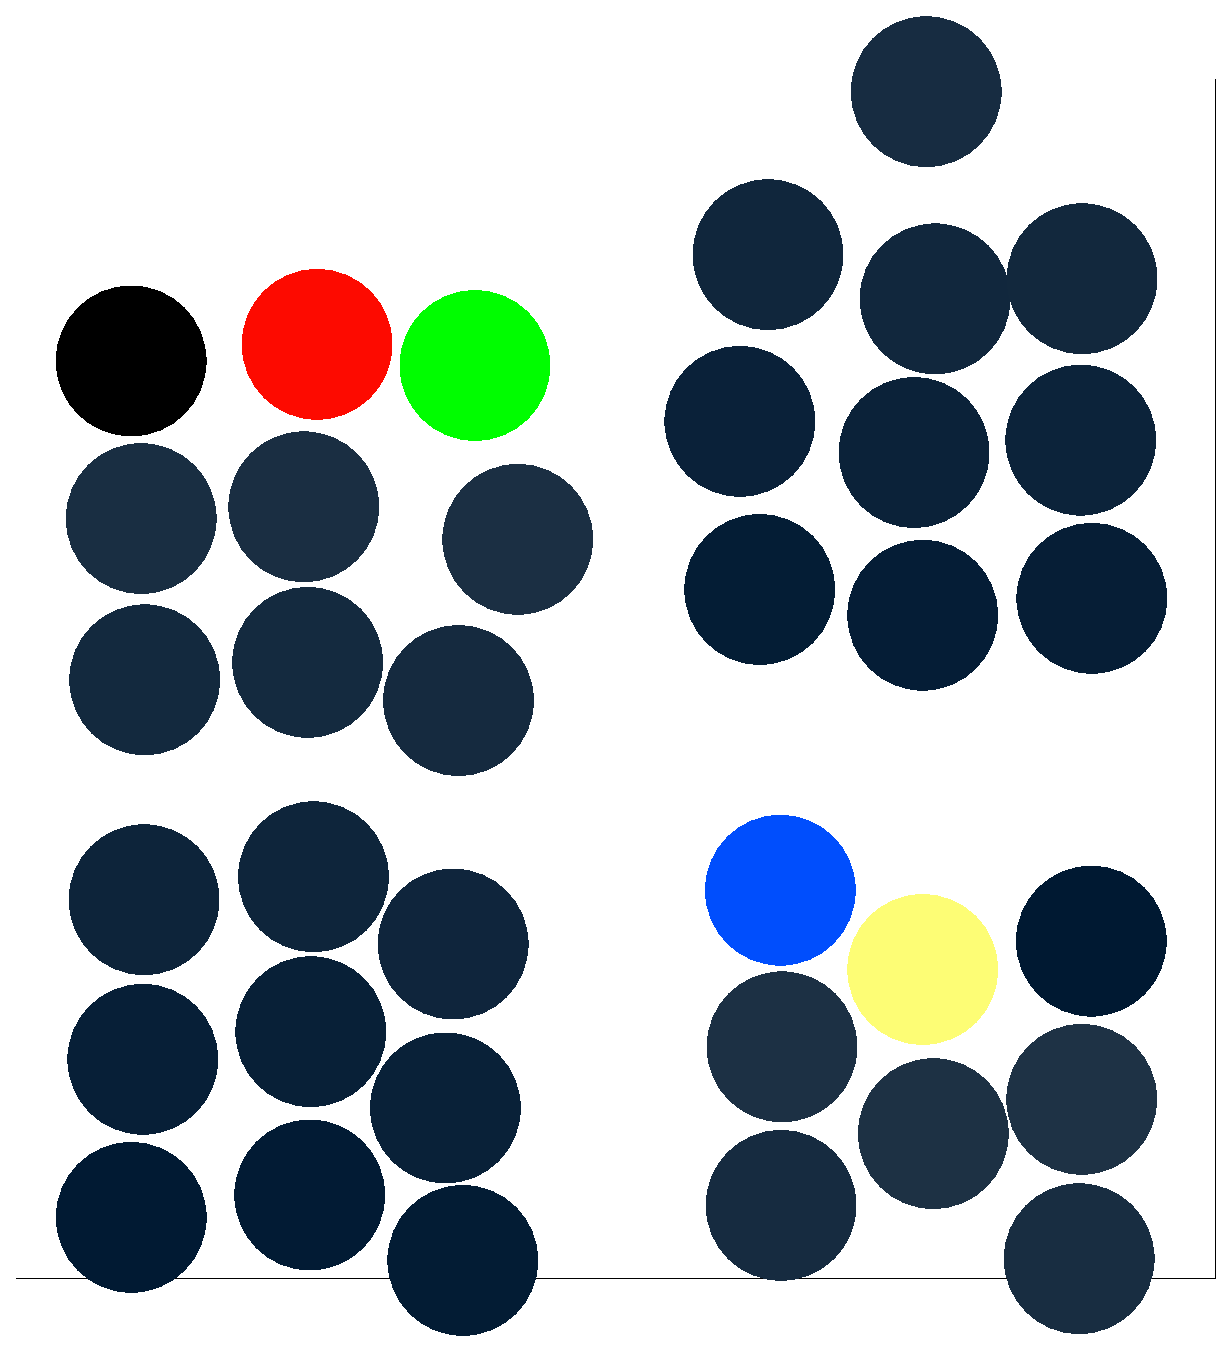
\includegraphics[width=0.19\textwidth]{graph3d_015.eps}
  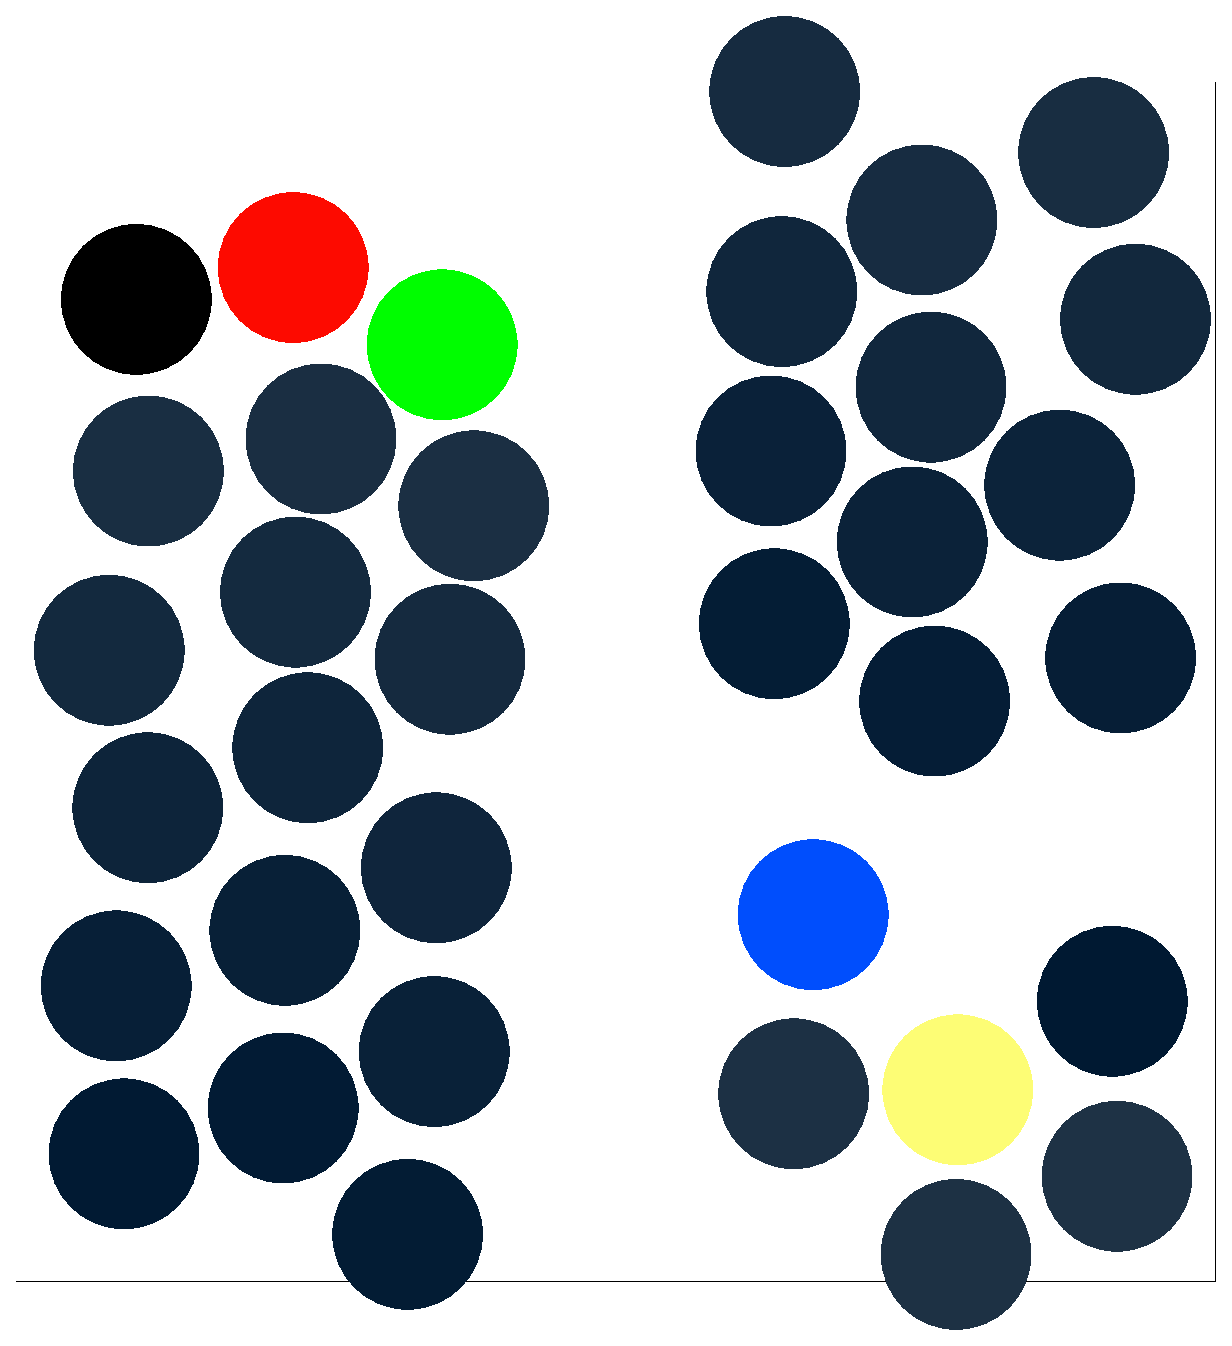
\includegraphics[width=0.19\textwidth]{graph3d_016.eps}
  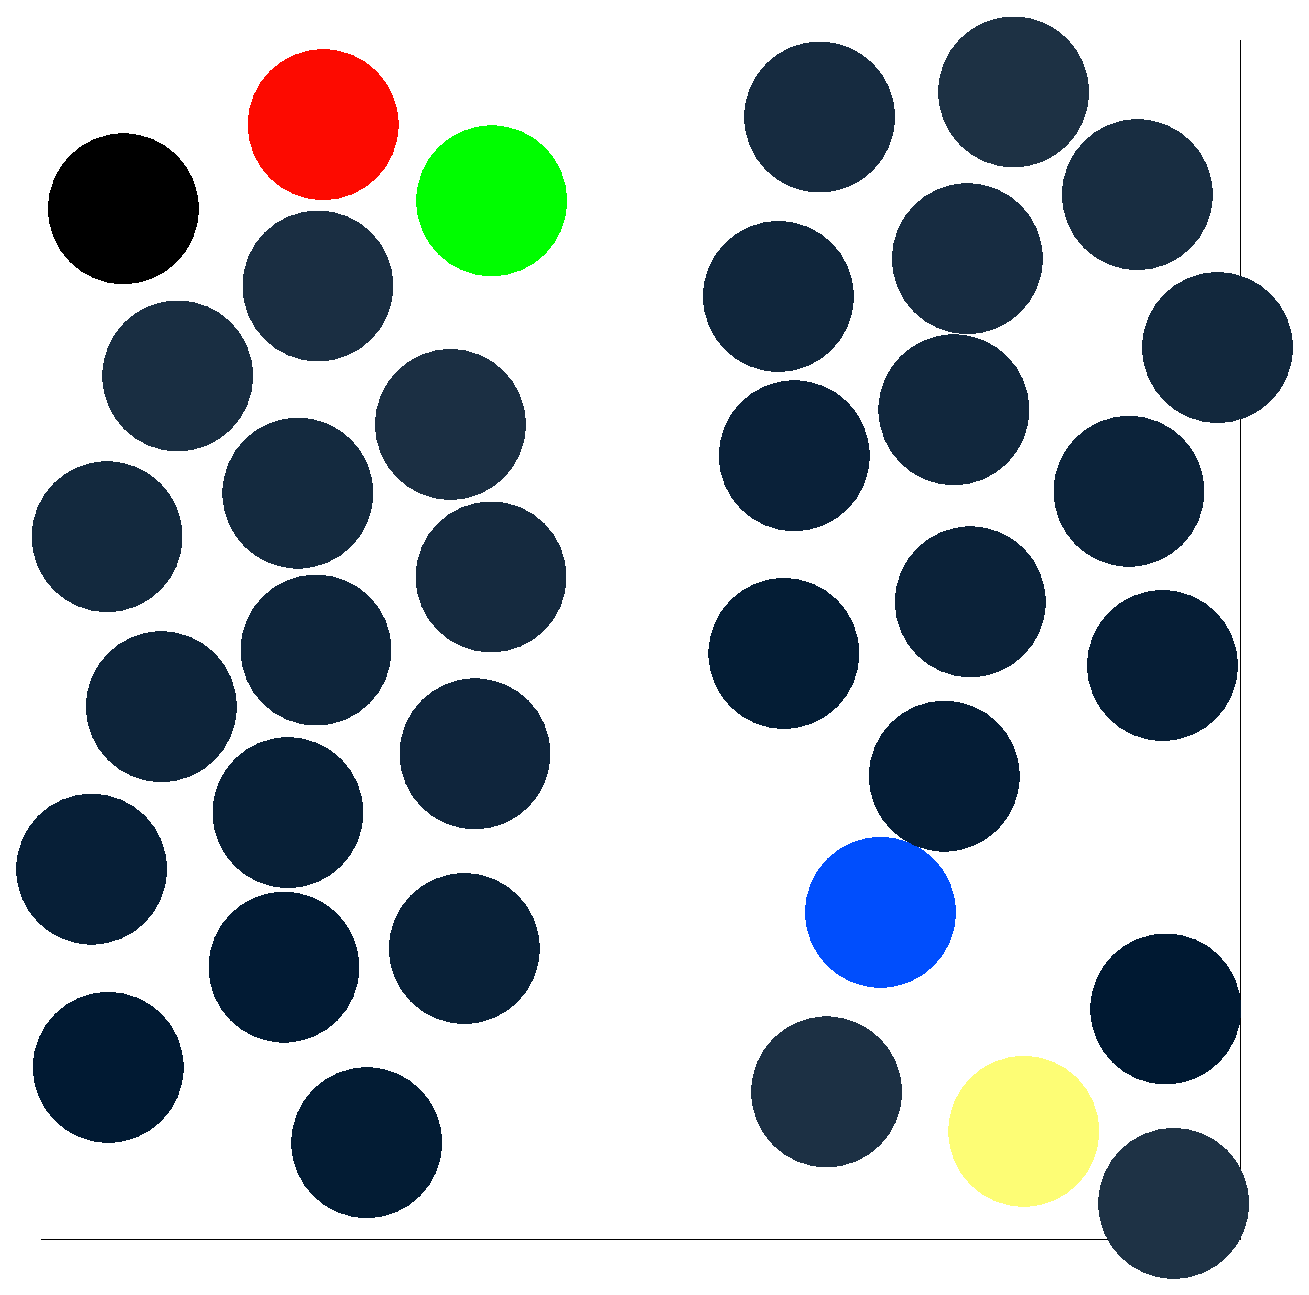
\includegraphics[width=0.19\textwidth]{graph3d_017.eps}
%  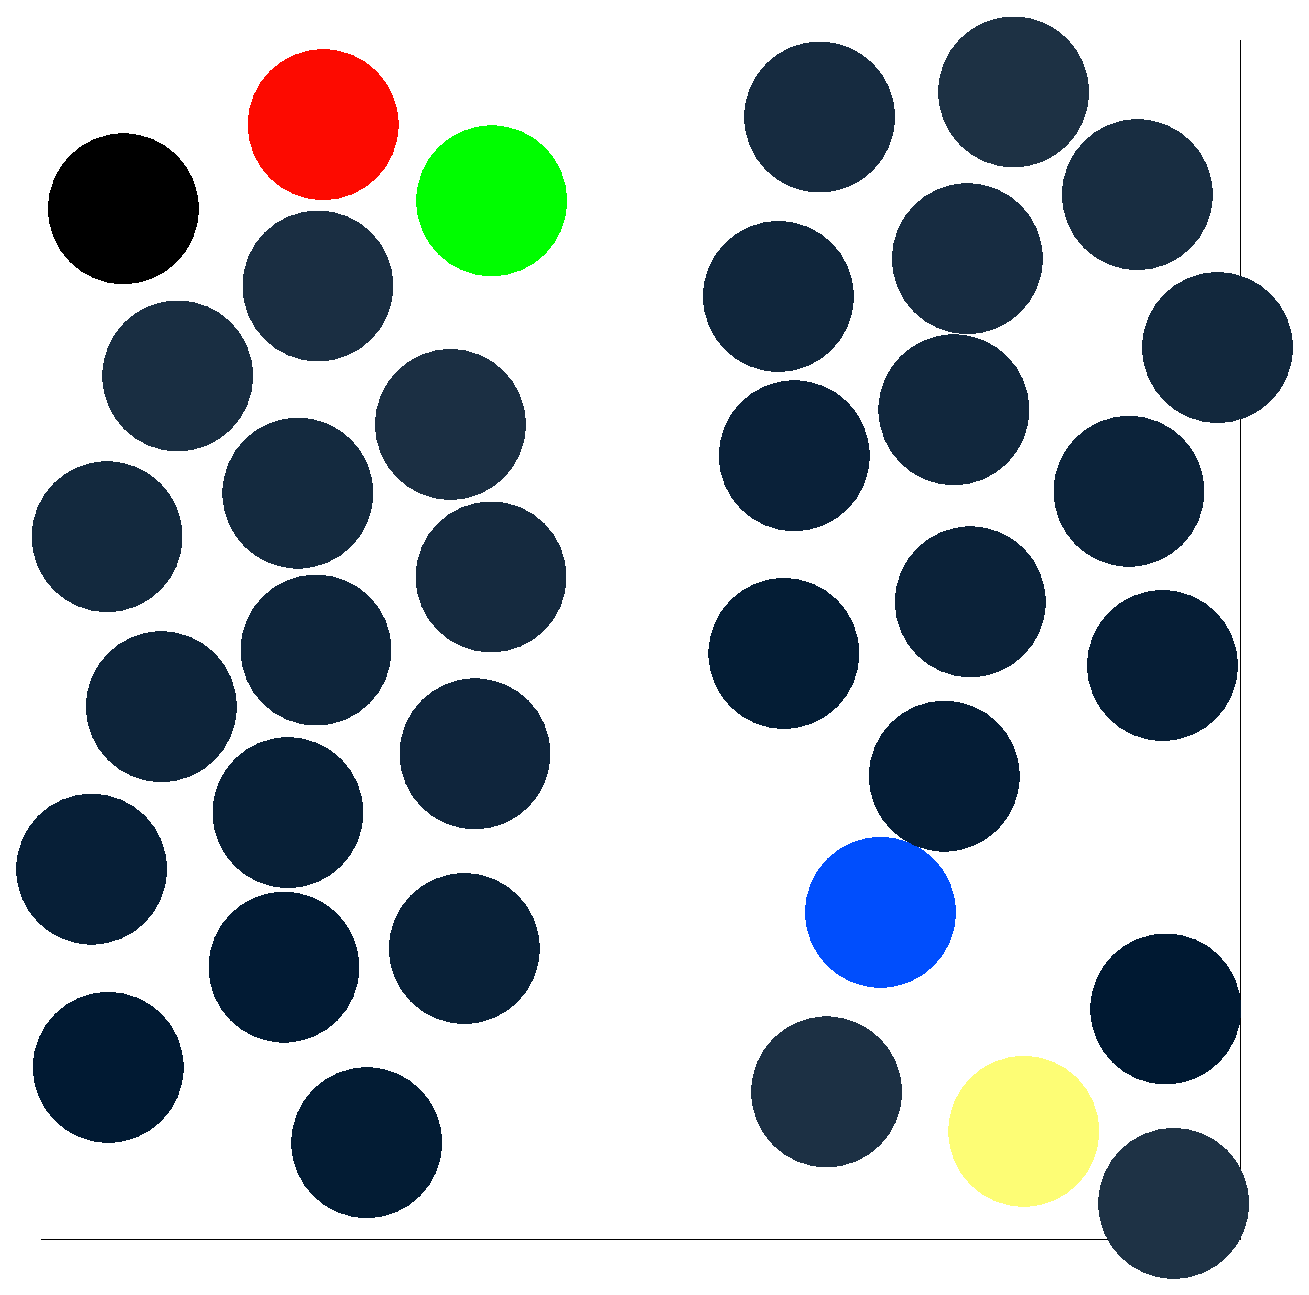
\includegraphics[width=0.19\textwidth]{graph3d_018.eps}
  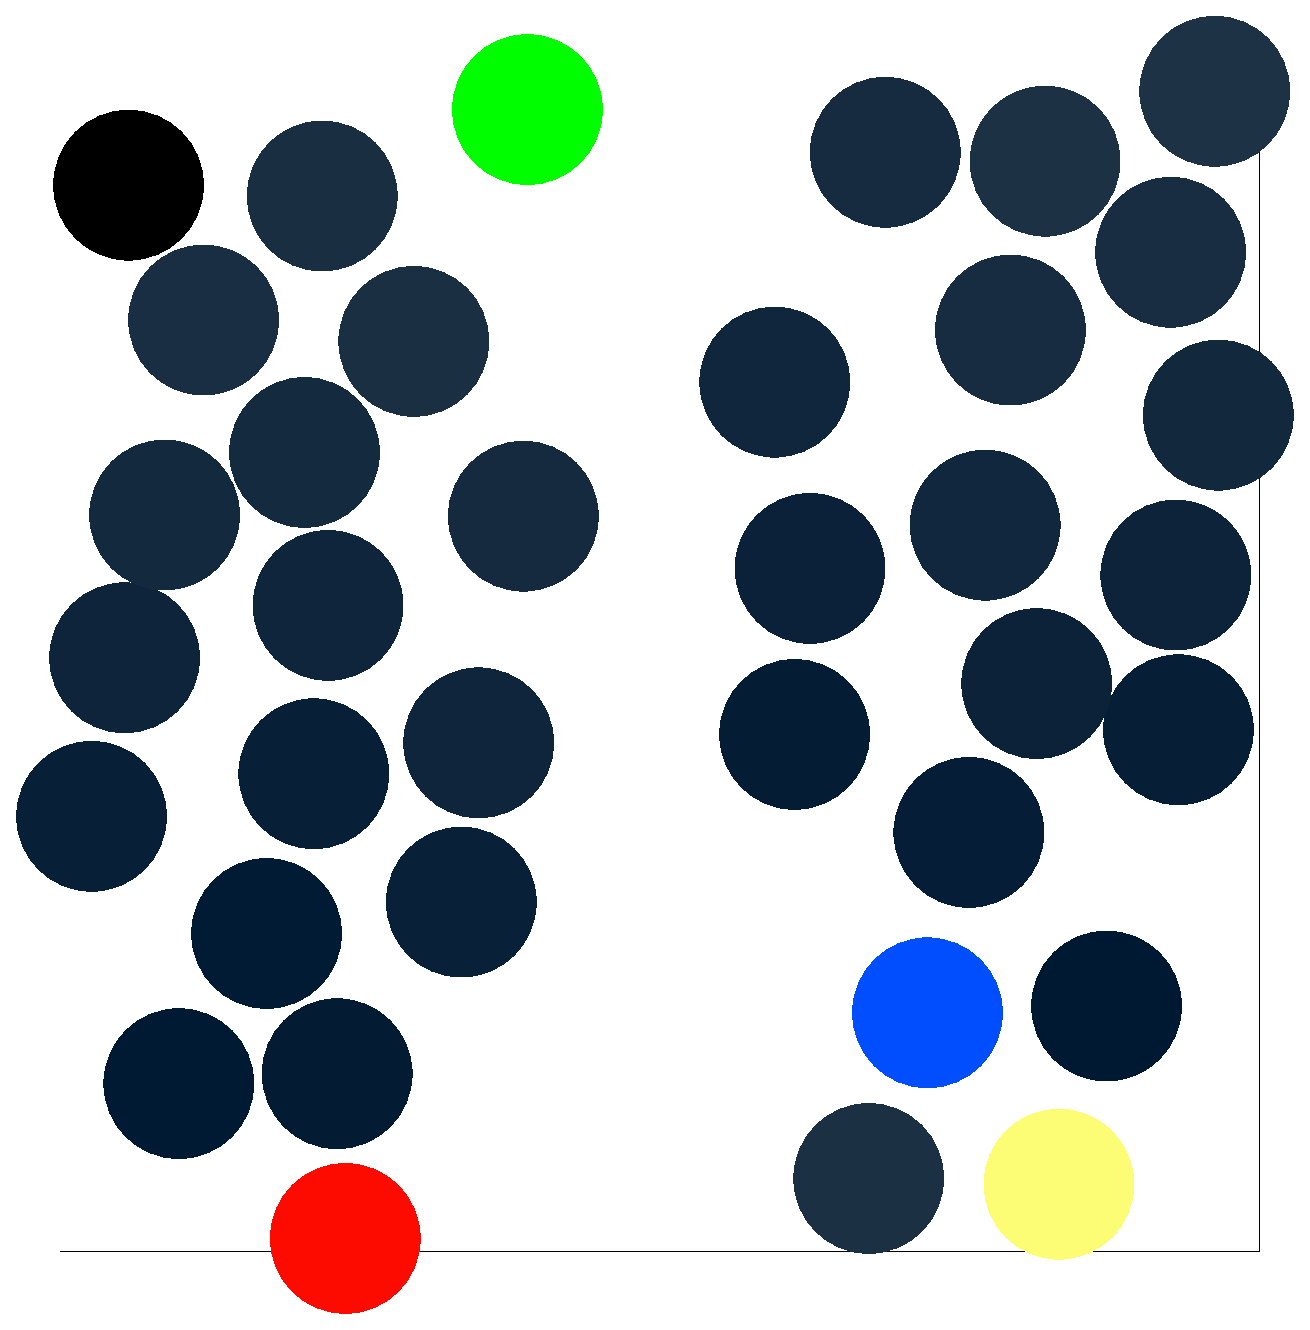
\includegraphics[width=0.19\textwidth]{graph3d_019.eps}
  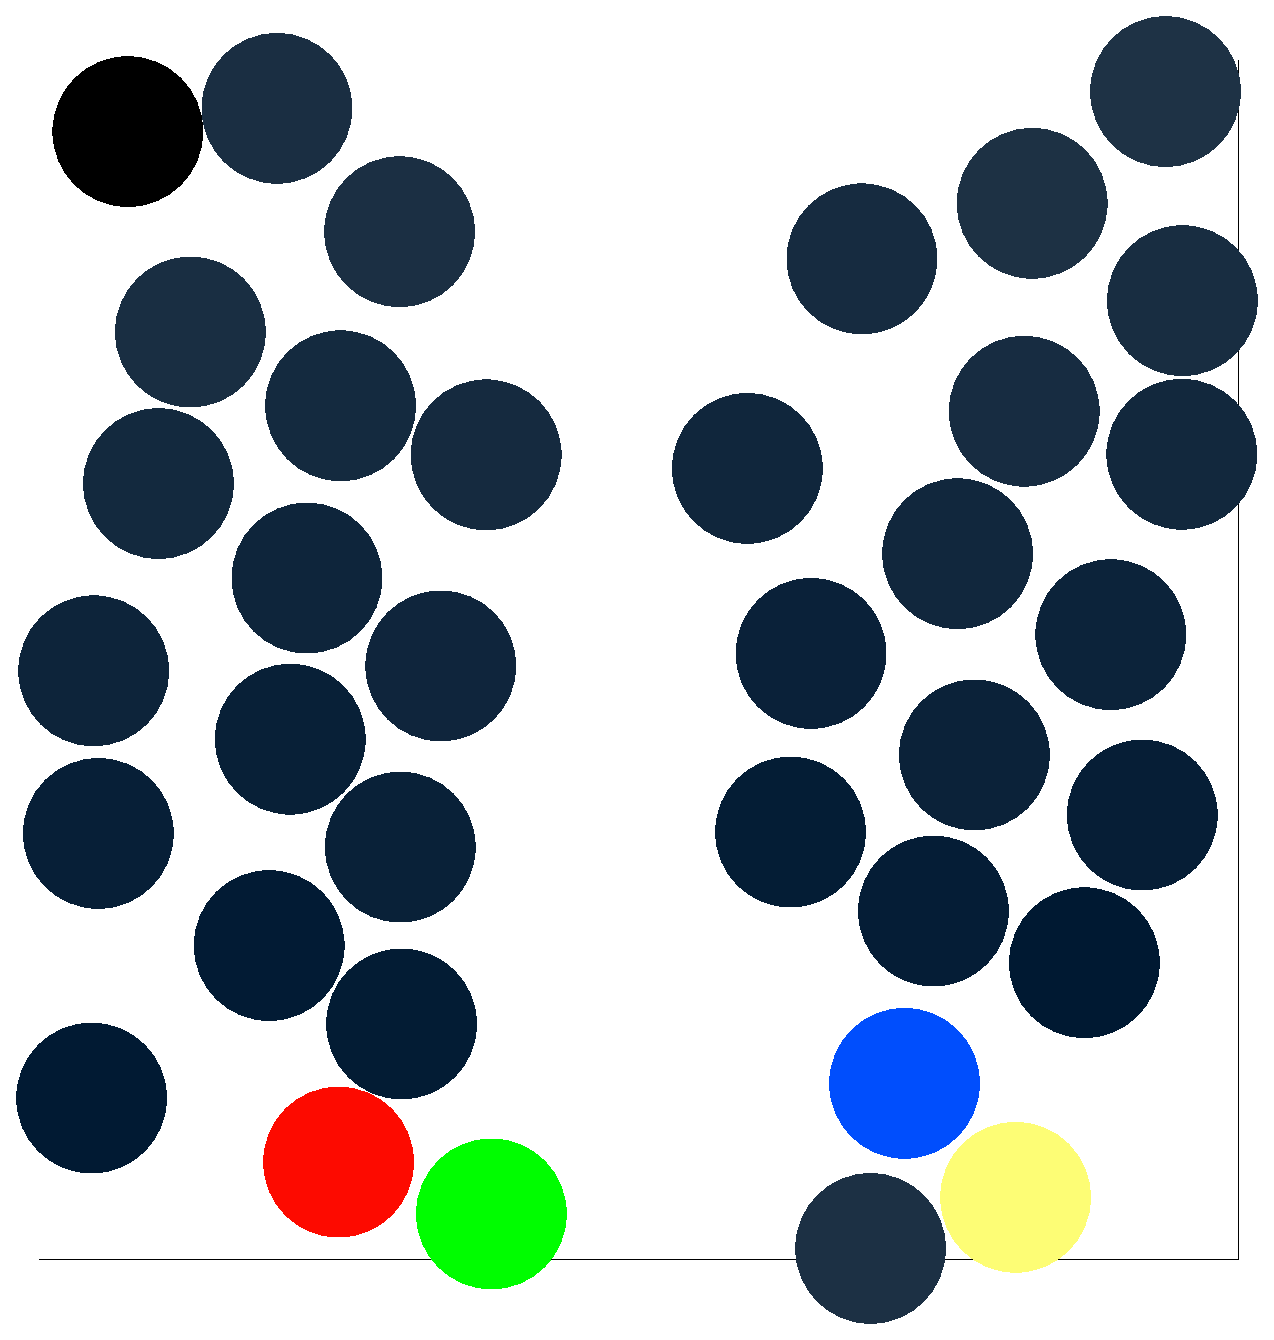
\includegraphics[width=0.19\textwidth]{graph3d_020.eps}
  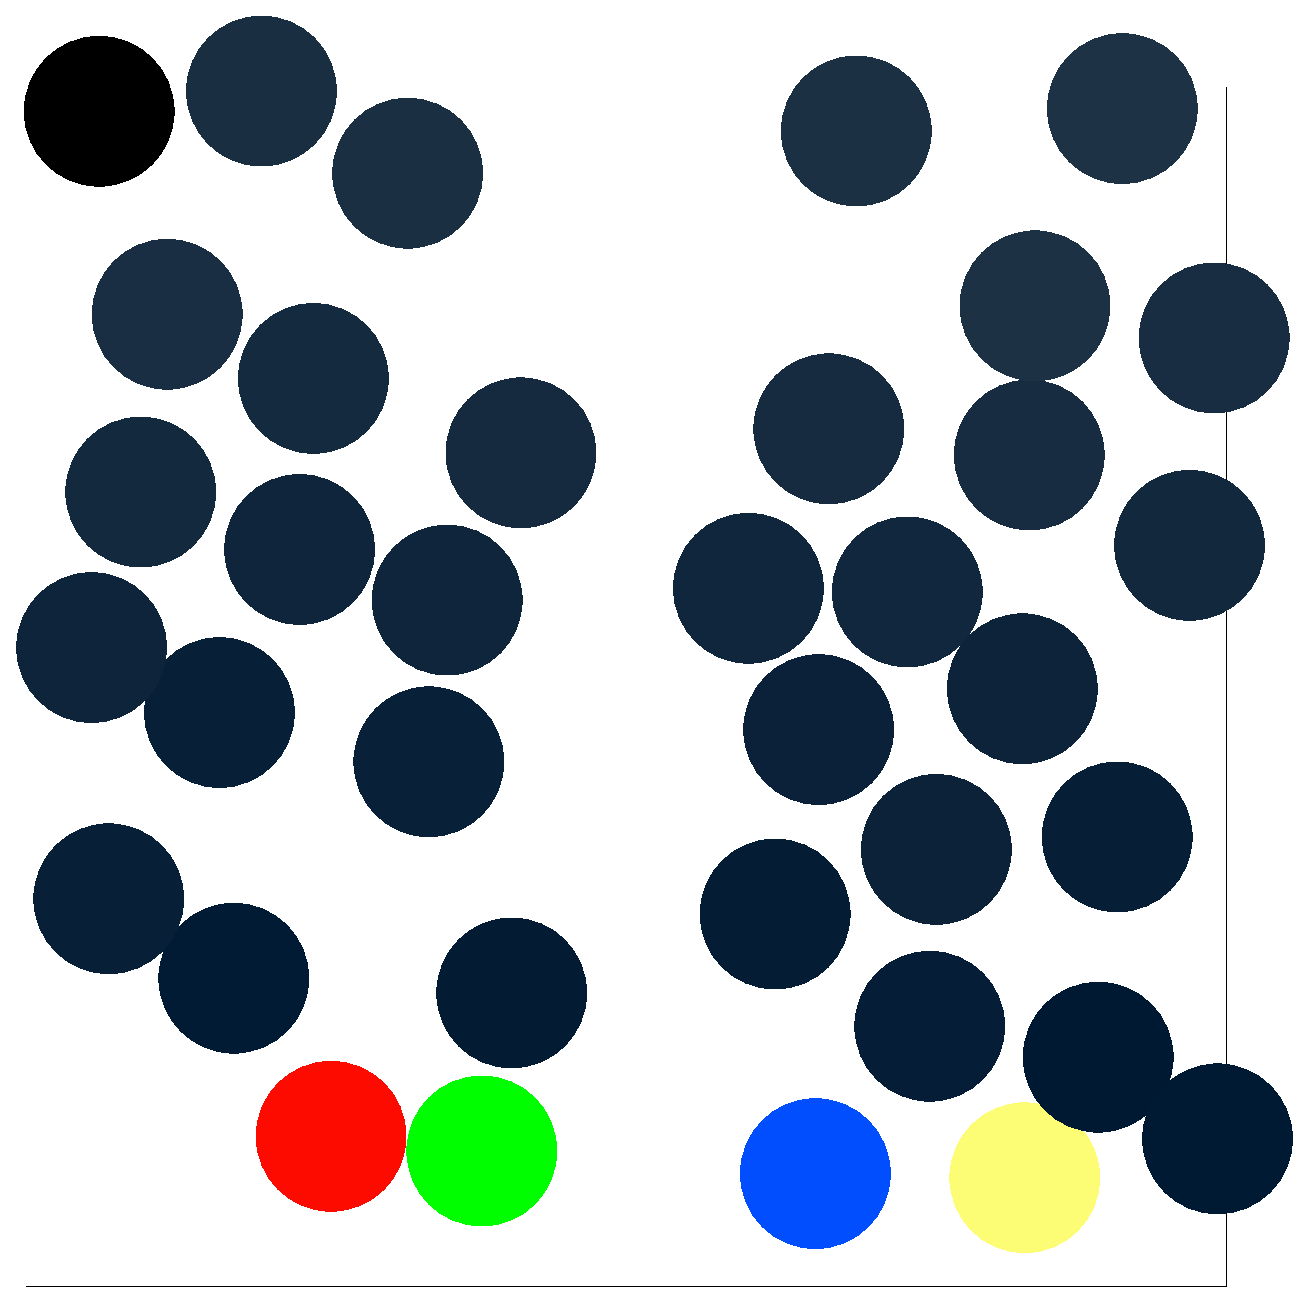
\includegraphics[width=0.19\textwidth]{graph3d_021.eps}
  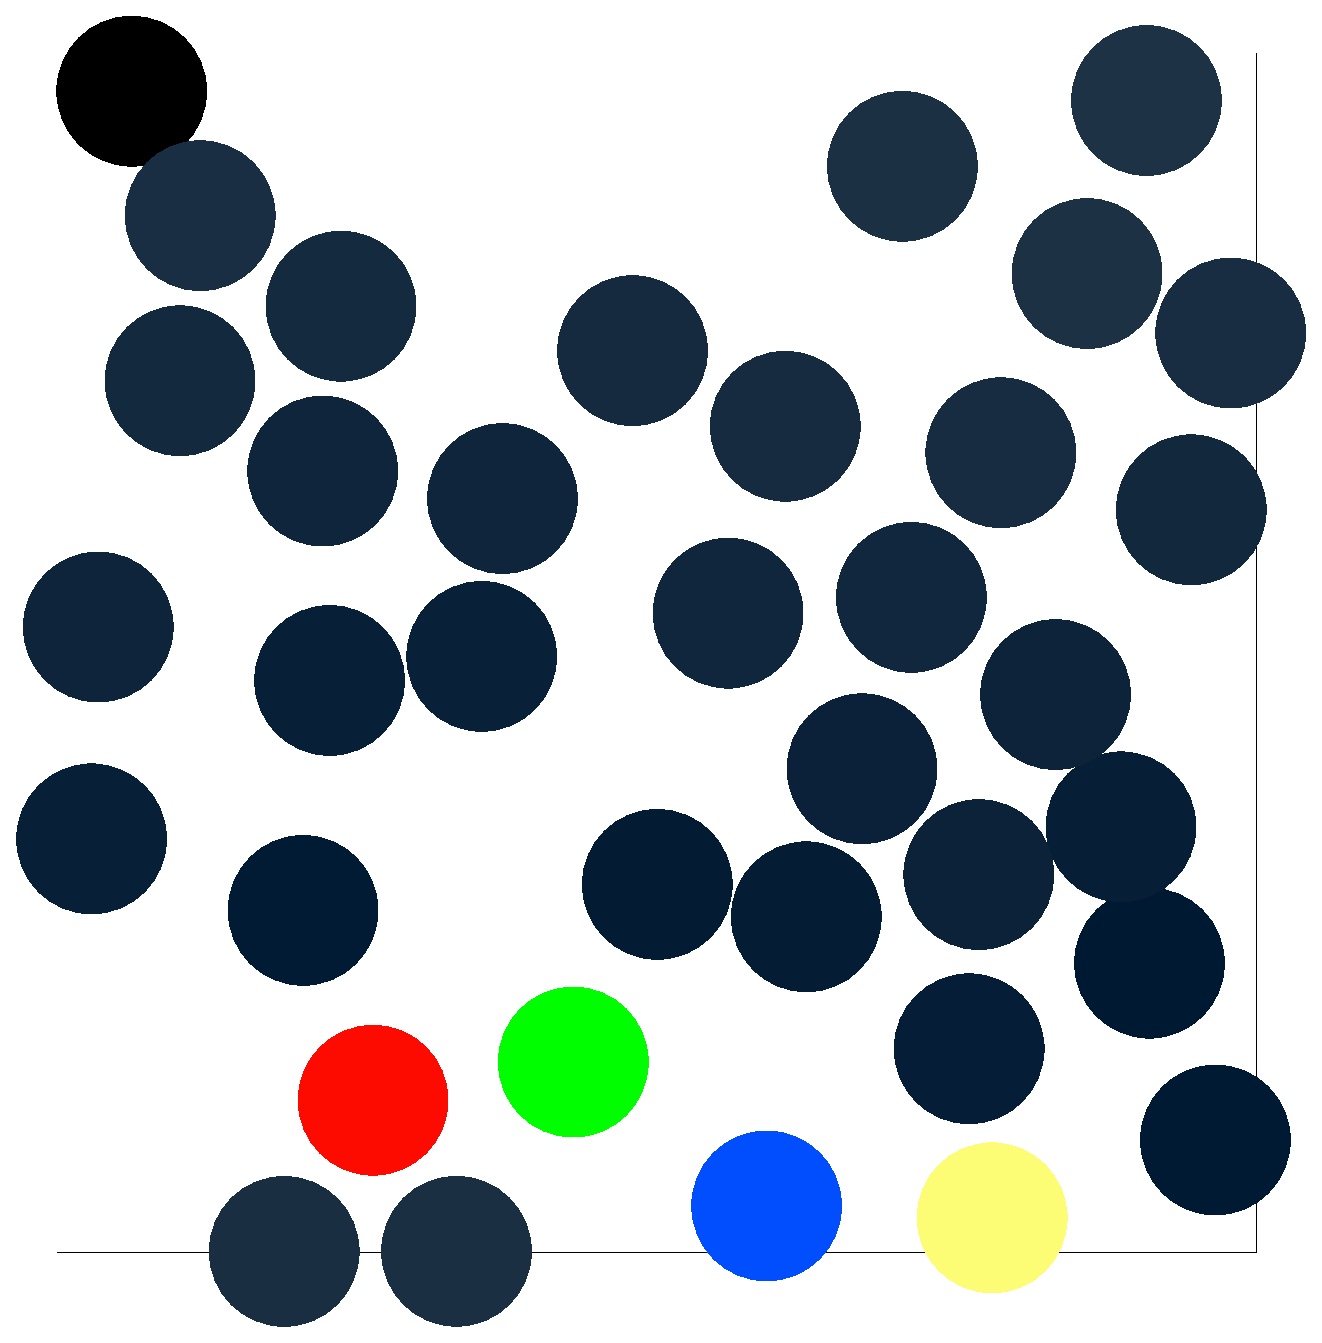
\includegraphics[width=0.19\textwidth]{graph3d_022.eps}
  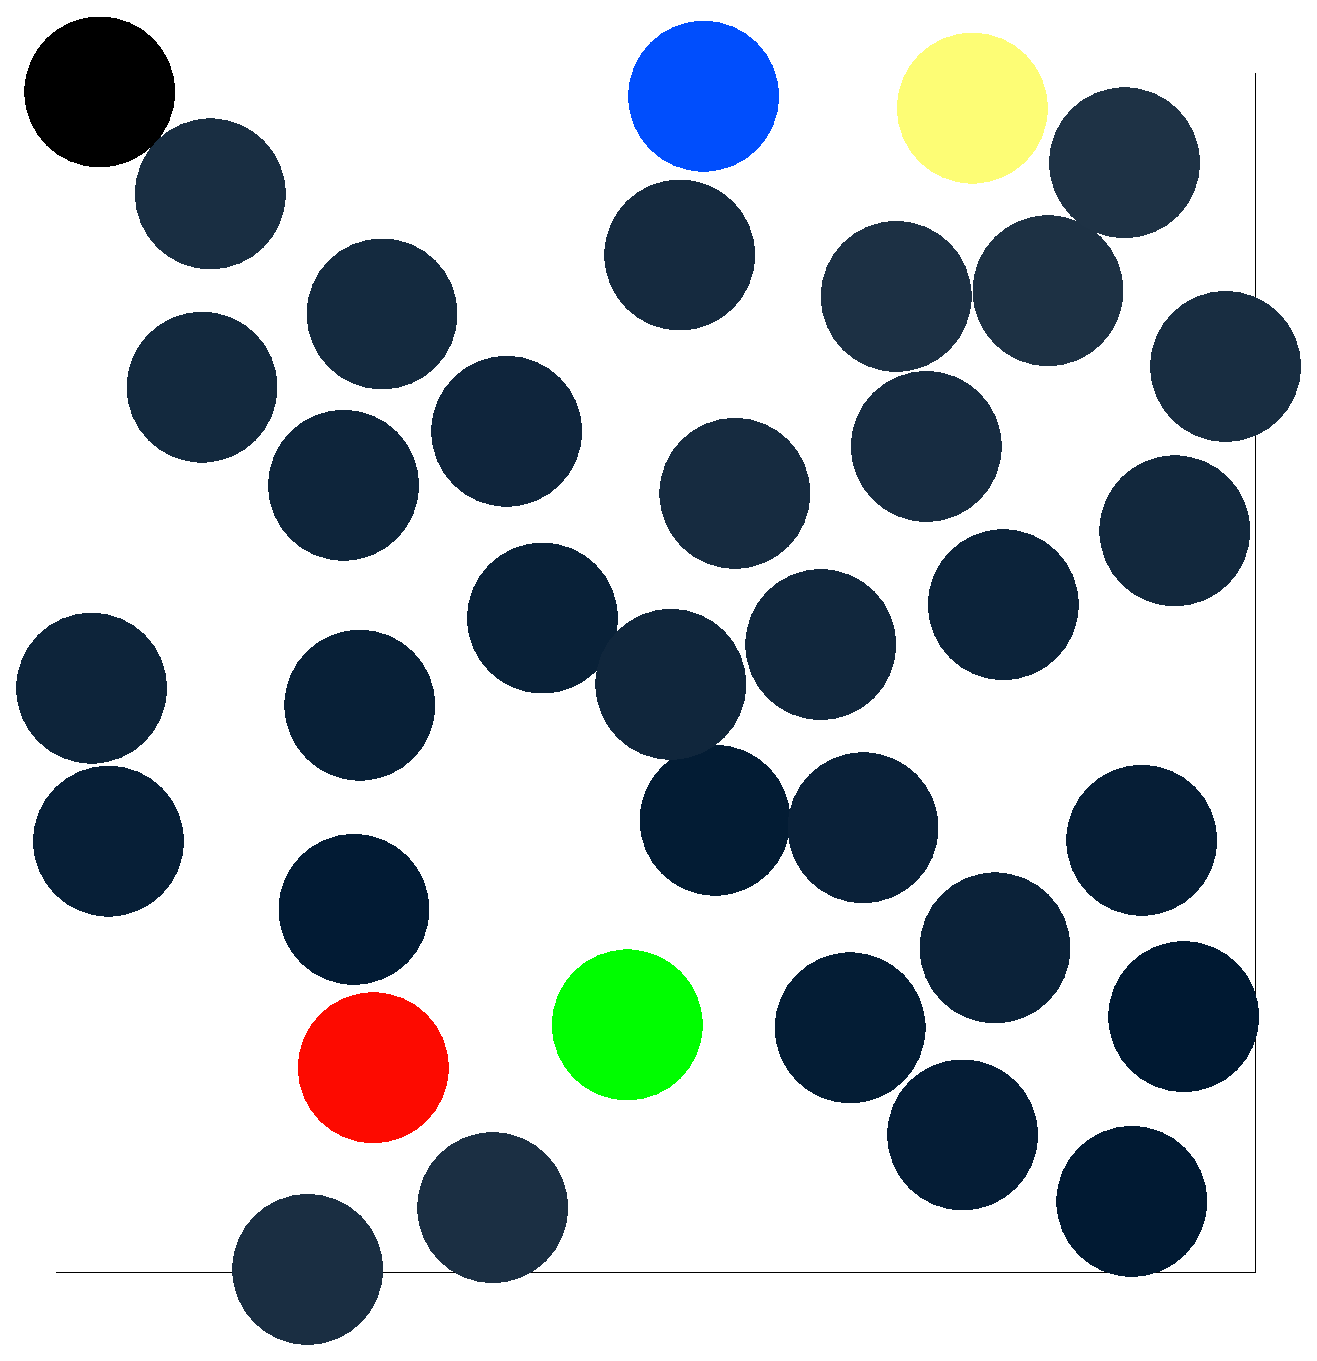
\includegraphics[width=0.19\textwidth]{graph3d_023.eps}
  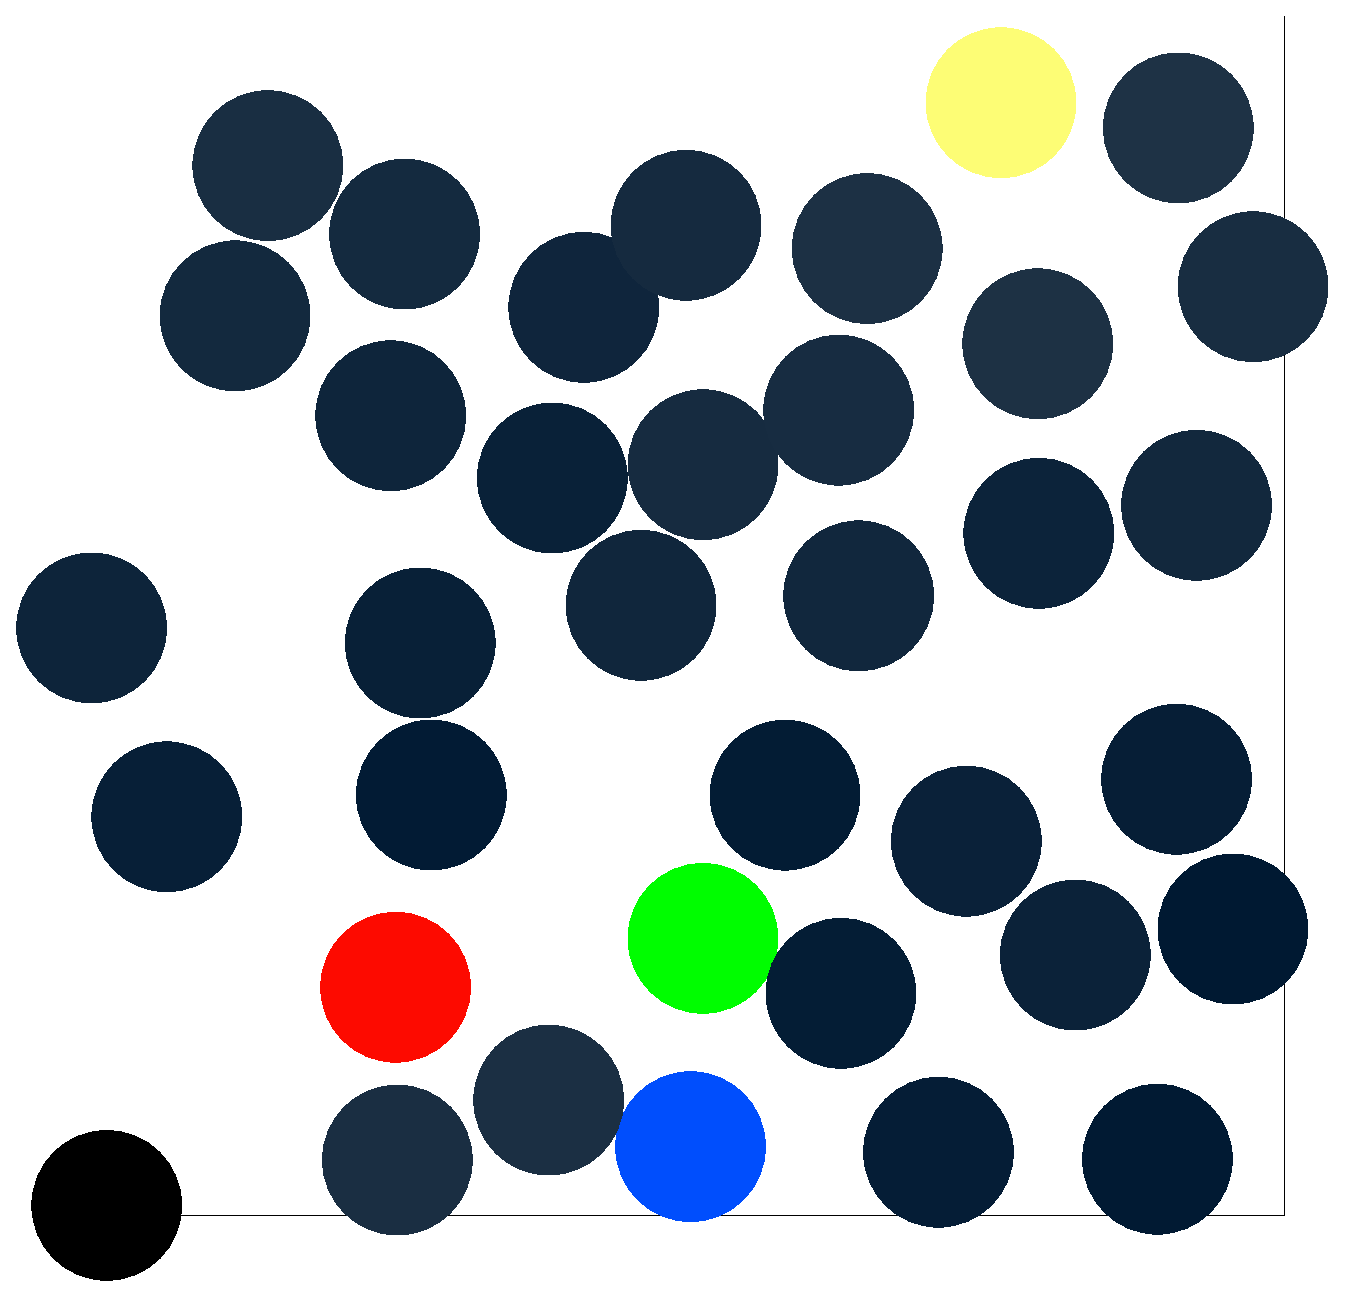
\includegraphics[width=0.19\textwidth]{graph3d_024.eps}
  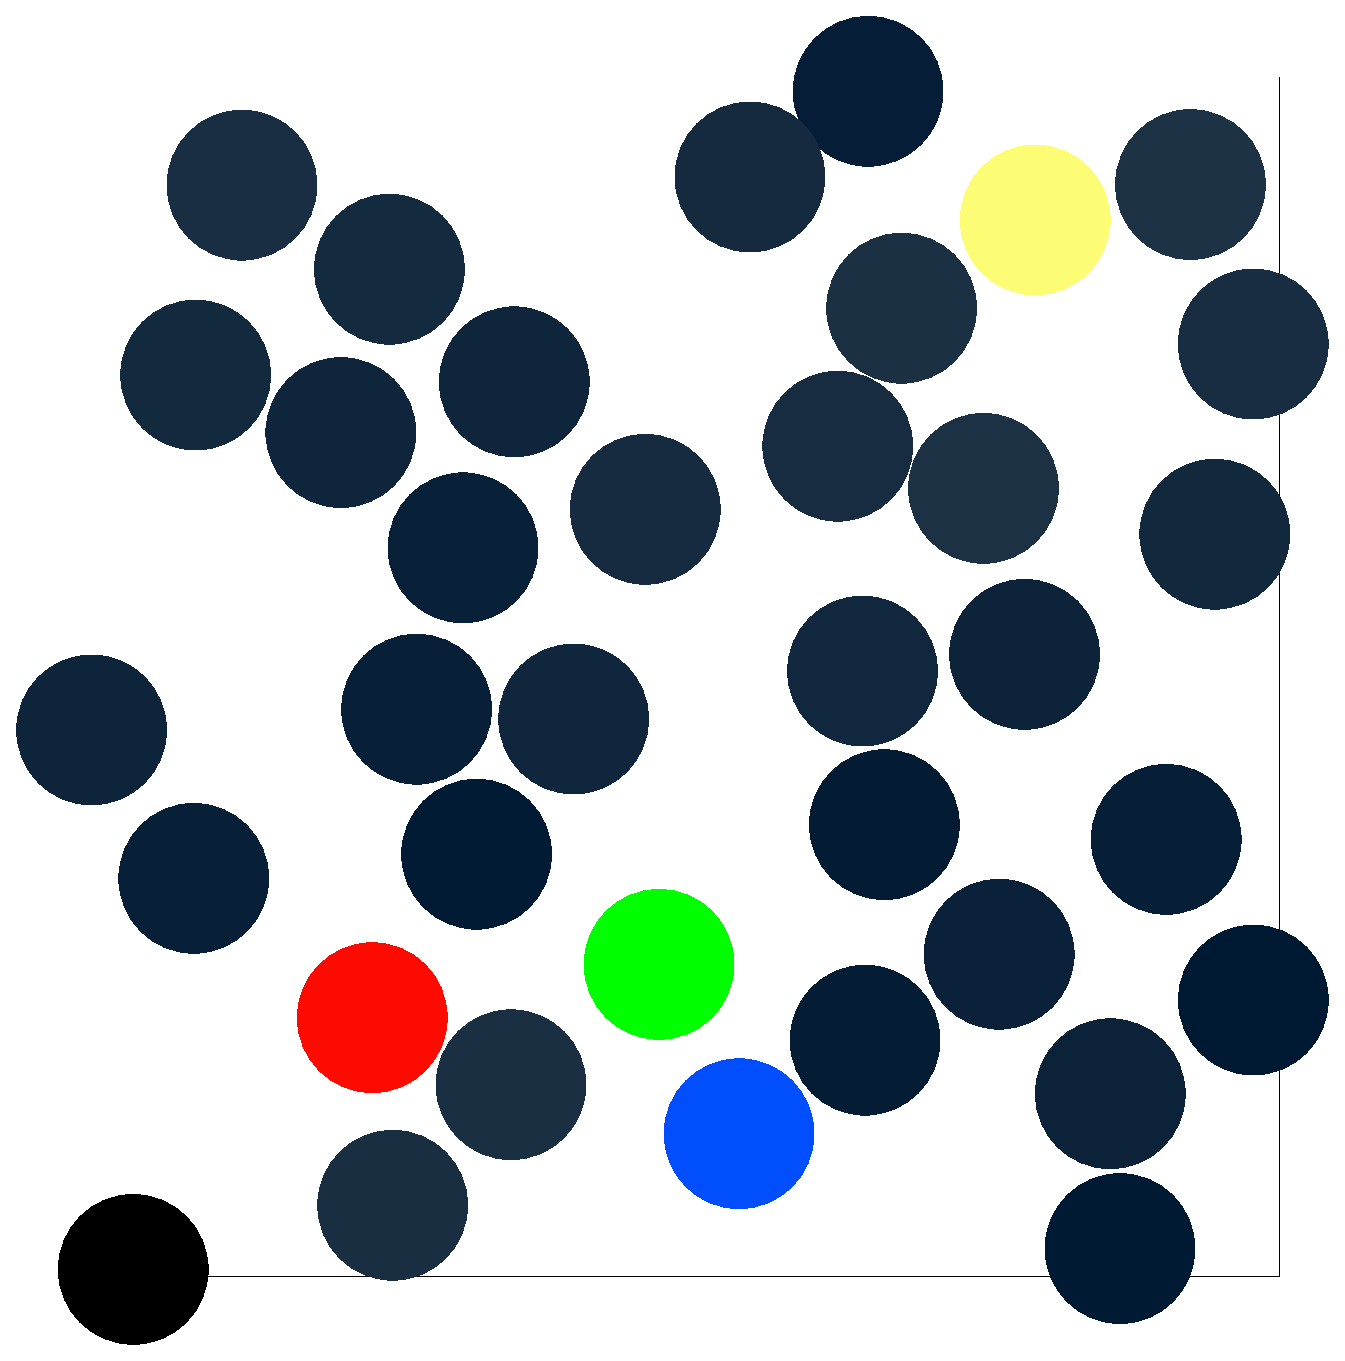
\includegraphics[width=0.19\textwidth]{graph3d_025.eps}
  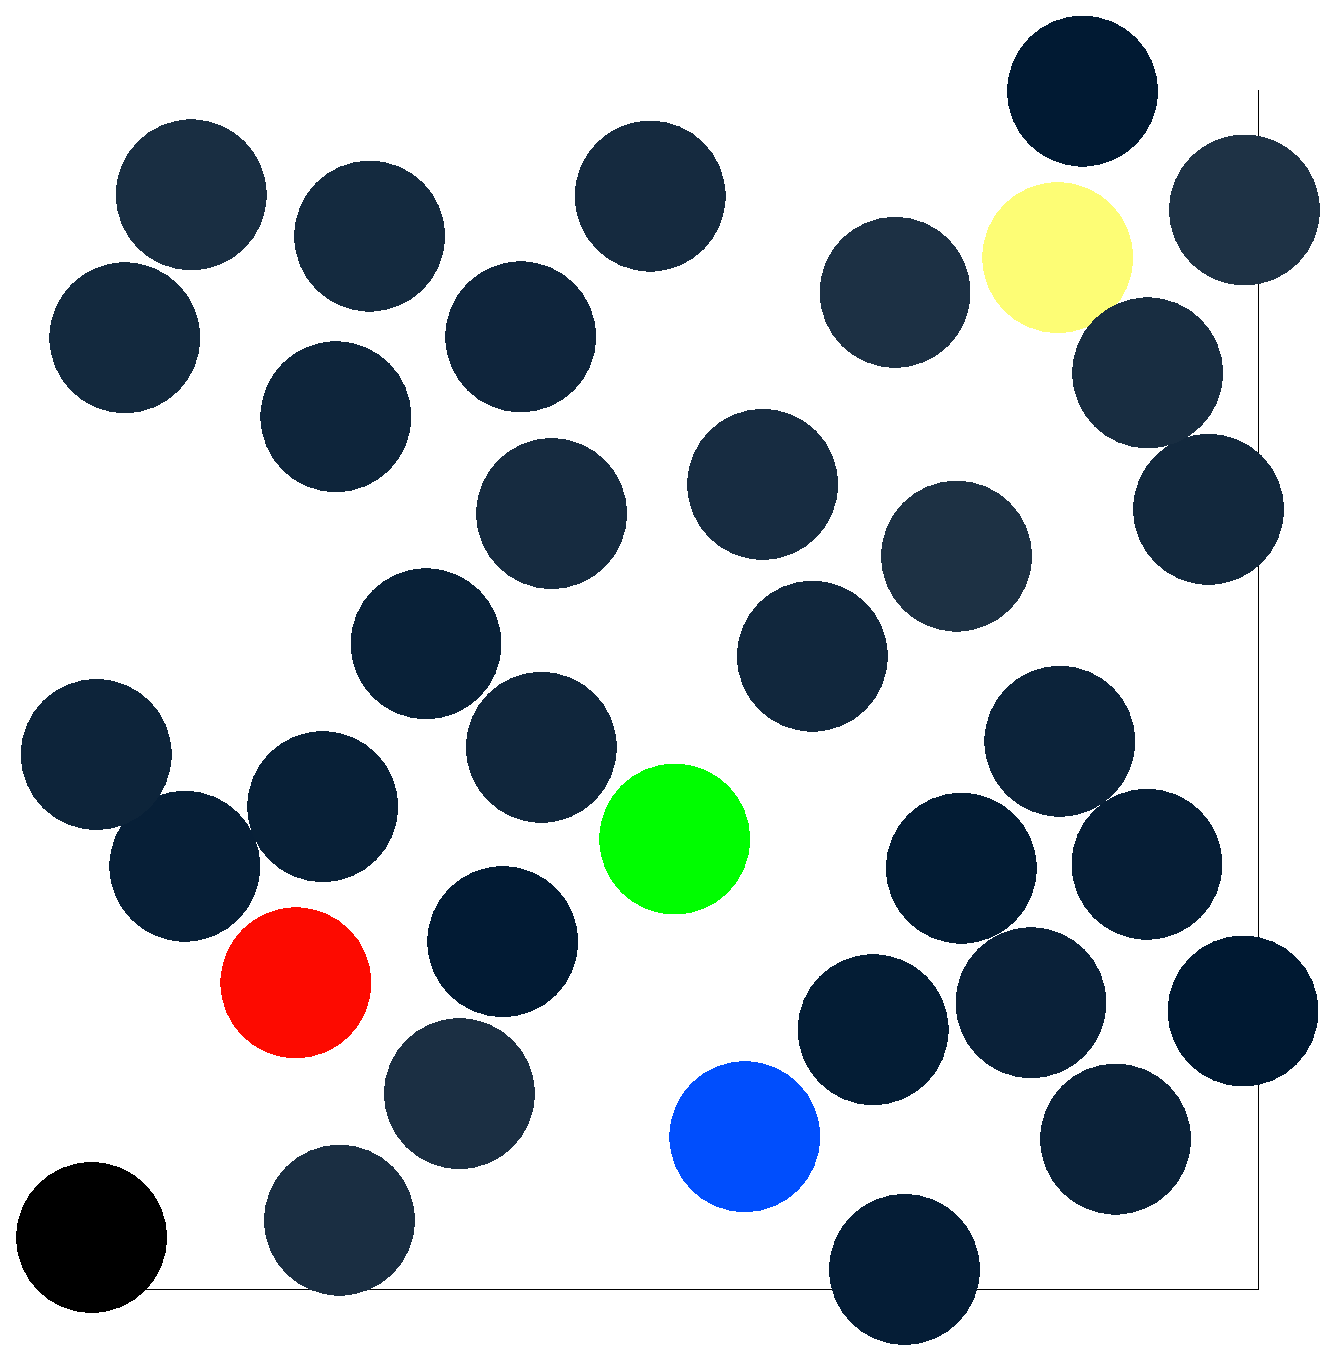
\includegraphics[width=0.19\textwidth]{graph3d_026.eps}
  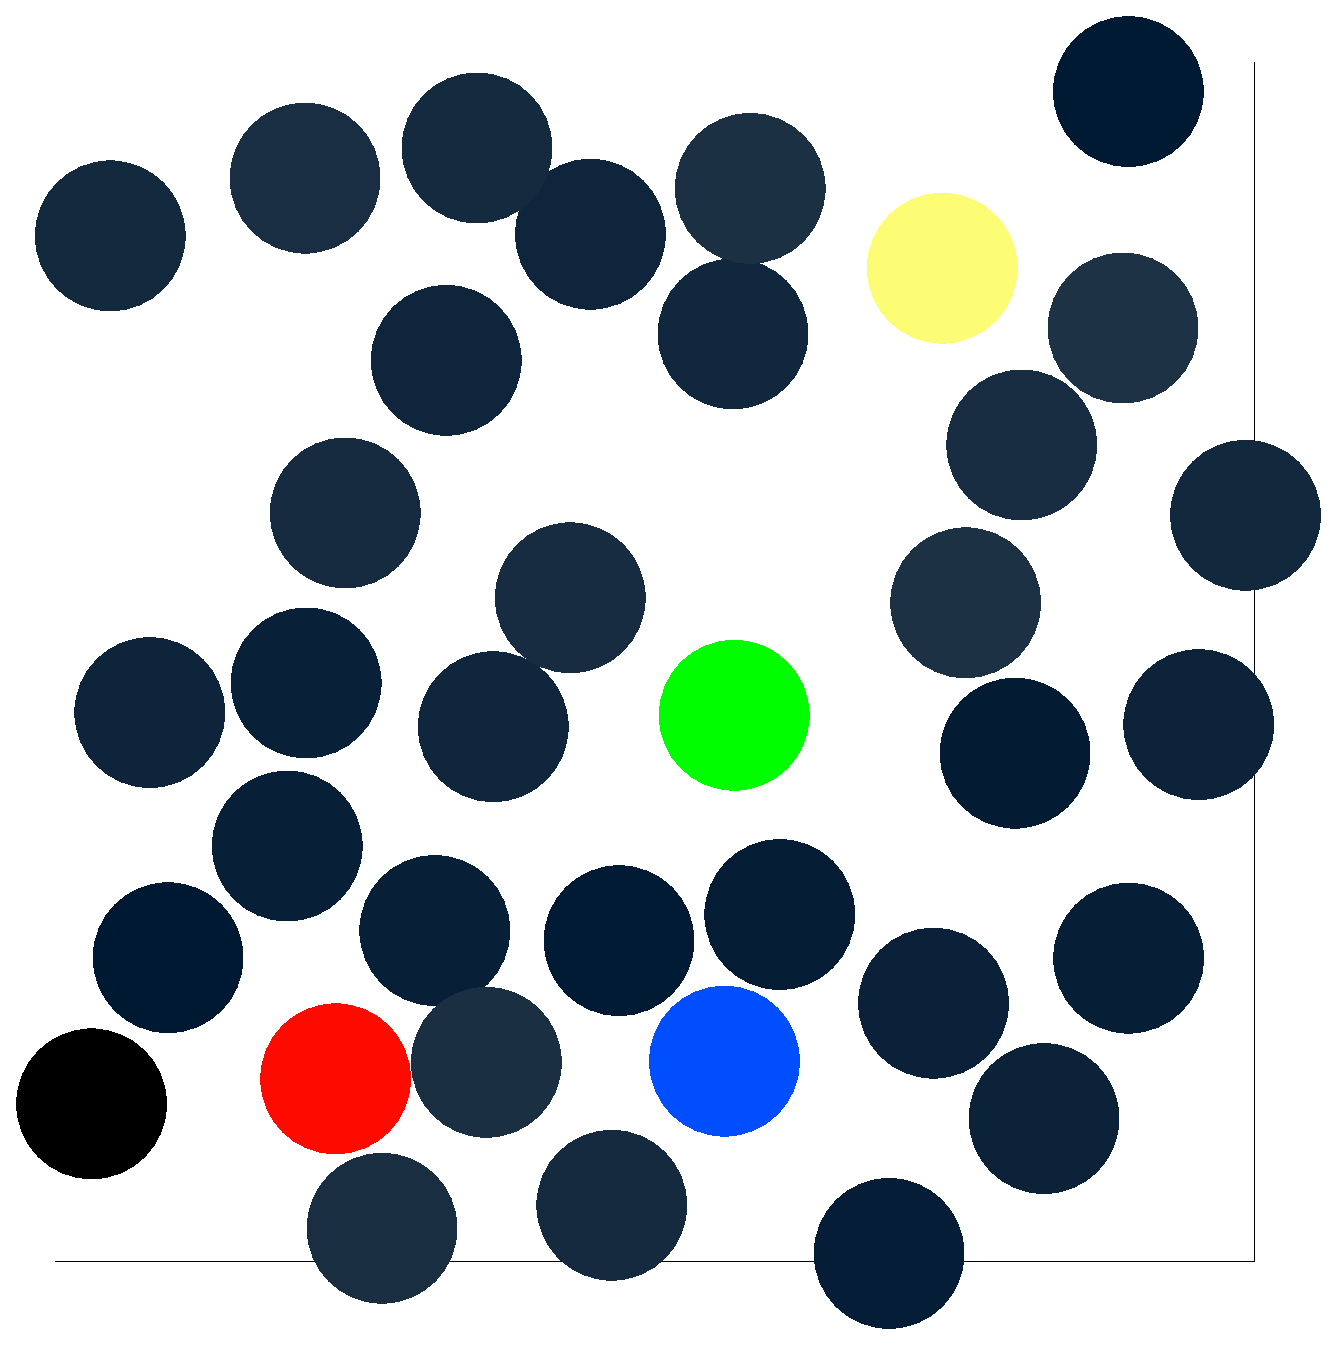
\includegraphics[width=0.19\textwidth]{graph3d_027.eps}
  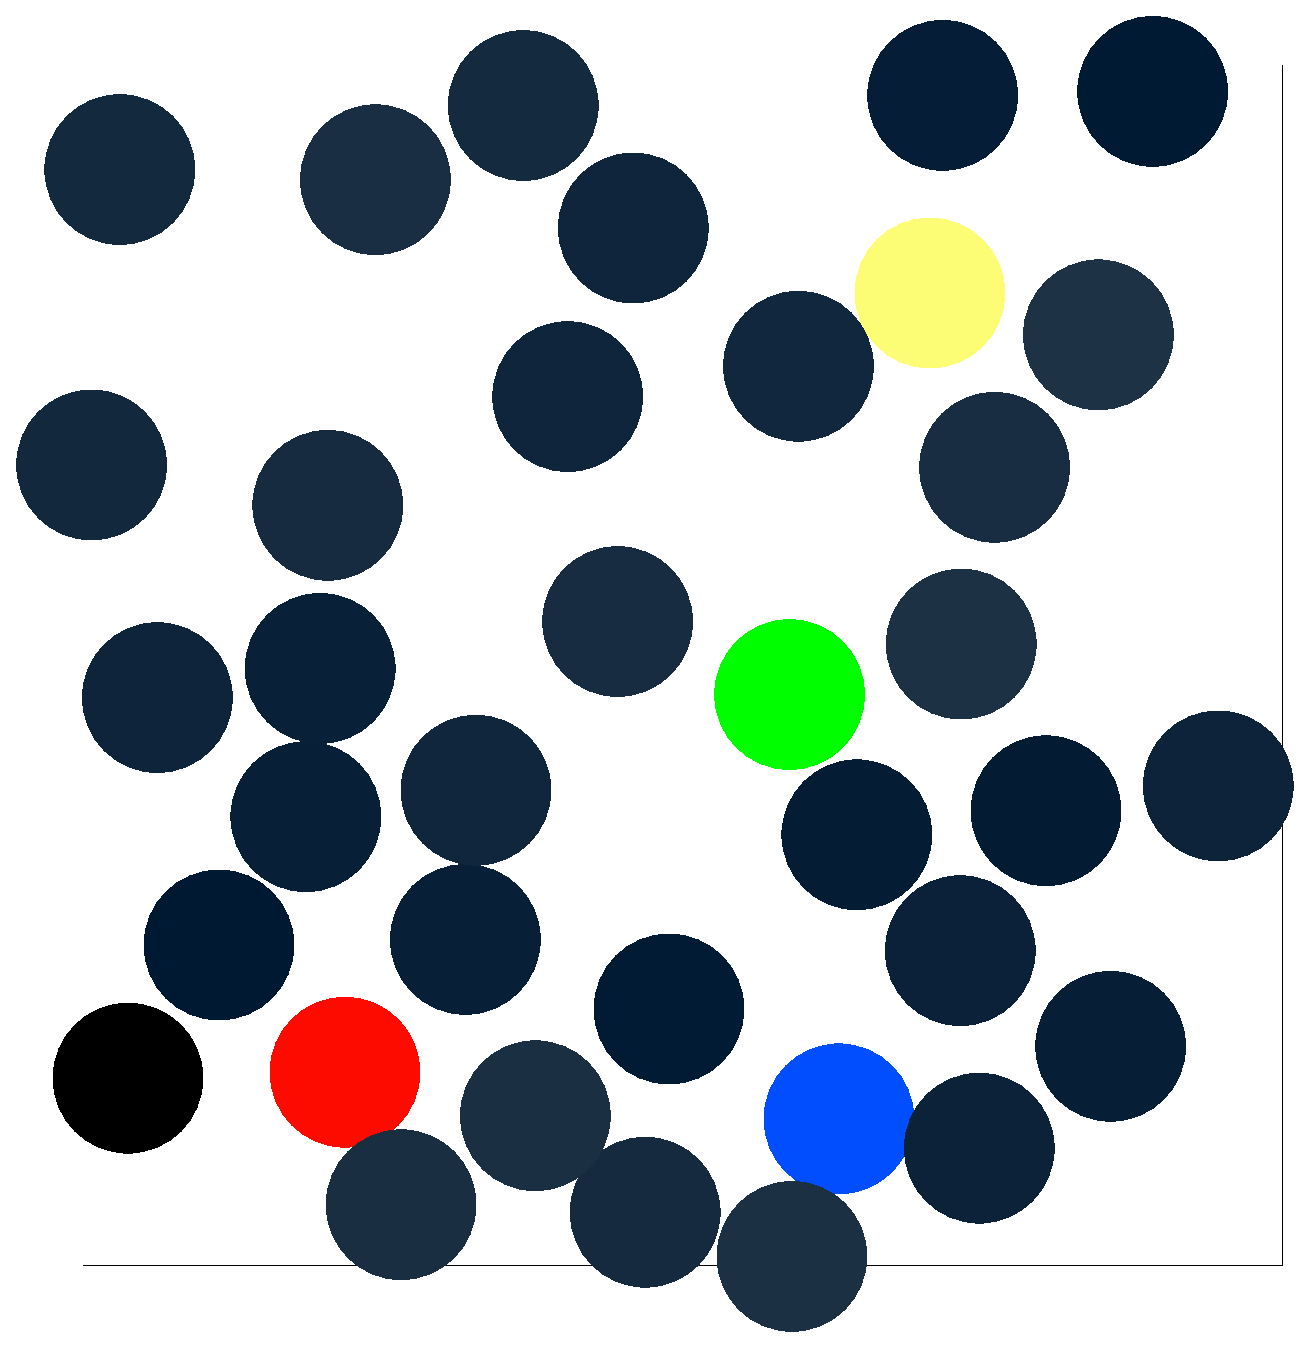
\includegraphics[width=0.19\textwidth]{graph3d_028.eps}
%  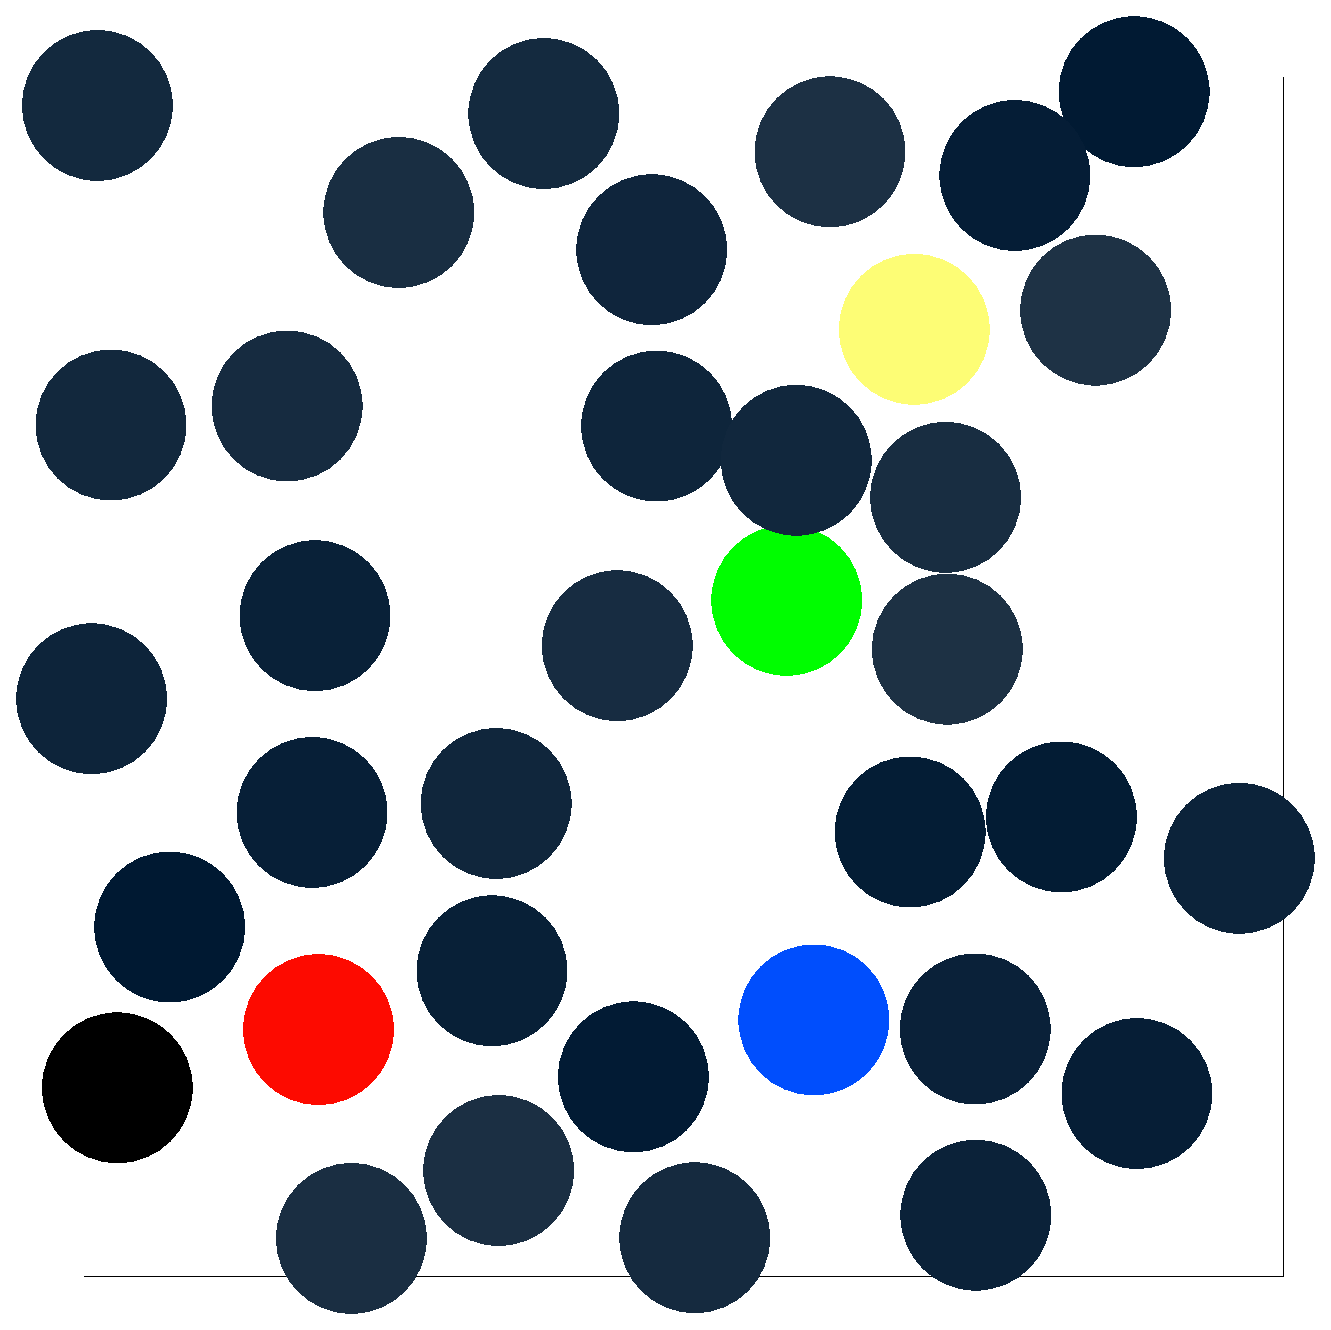
\includegraphics[width=0.19\textwidth]{graph3d_029.eps}
\caption{\label{fig2} A sample output for a system with $L=8$ and 36 particles arranged on a regular square lattice. The particles move in unison for a while until computational errors break the initial symmetry. The time-step was $\Delta t=0.01$ and we show subsequent results after 50 iterations.}
\end{figure}

These simulations show that particles reenter at the boundaries of the simulation and that no spurious effects are obvious at the periodic boundaries.

\section{Conclusions}
In this report we have shown how to implement periodic boundary conditions in a Molecular Dynamics simulation. We have verified that our algorithm is free from obvious errors by setting up a periodic system and observing that it shows no spurious edge effects.


\appendix
\section{Code}
%\includecode[C]{/home/david/Documents/Computational_Physics/MD.c}
\end{document}
  
